\documentclass[11pt]{article}

\usepackage[margin=1in]{geometry}
\usepackage{amsmath,amssymb}
\usepackage{graphicx}
\usepackage{booktabs}
\usepackage{xcolor}
\usepackage{hyperref}
\hypersetup{colorlinks=true, linkcolor=blue, citecolor=blue, urlcolor=blue}
\usepackage{caption}
\usepackage{authblk}

\newcommand{\SBA}{S(B|A)}
\newcommand{\NMI}{\mathrm{NMI}}
\newcommand{\Strue}{S_{\rm true}}
\newcommand{\Itrue}{I_{\rm true}}

\title{Quantum vs.\ Classical Correlations in Dijet Hadron Multiplicities:\\
A Finite-Statistics Methodology Note}

\author[1,2]{Zhoudunming (Kong) Tu}
\affil[1]{Brookhaven National Laboratory}
\affil[2]{Stony Brook University}

\date{\today}

\begin{document}
\maketitle

\begin{abstract}
\noindent
We develop and validate a complete methodological pipeline for measuring
mutual information (MI), conditional entropy $\SBA$, and a normalized
witness $\NMI=I(A{:}B)/\min(S_A,S_B)$ between back-to-back jet hadron
multiplicities, testing whether an observed dijet correlation is
classically explicable or could signal genuine quantum entanglement. The
naive plug-in entropy estimator is biased upward at finite sample size,
in exactly the direction that could mimic a quantum excess; using a
Monte Carlo toy model with known ground truth, we validate two standard
corrections (Miller--Madow, shuffle-subtraction) and a Bayesian
estimator (NSB), and derive a quantitative detection-sensitivity curve
from the best-behaved of these. The full pipeline, cross-validated
between independent Python and ROOT/C++ implementations, is applied to
realistic PYTHIA~8 dijet Monte Carlo. Since PYTHIA output carries no
independently known true MI, we develop a closure test that calibrates
a synthetic model to the data's own statistics; applied to a full
validation sample this finds NSB's bootstrap uncertainty under-covers
by roughly $1.5$--$1.7\times$, improving substantially when the same
test is run separately within $p_T$ bins. We further identify and
correct a distinct systematic: any finite $p_T$ window induces real but
kinematically trivial MI, since both jets' multiplicities and their
$p_T$'s are correlated through momentum balance. A mixed-event
subtraction -- pairing each jet with a $p_T$-matched partner from a
different event -- isolates the beyond-kinematics MI; closure tests,
both on synthetic data and at full statistics on the real sample's own
fitted kinematics, show the naive estimator's finite-sample bias nearly
cancels between the same-event and mixed-event terms, so the raw
difference is close to unbiased even before rigorous correction.
Applied to the real validation sample, the subtraction finds a nonzero
beyond-kinematics component of order $0.003$~nats -- consistent across
all four estimator methods and plausibly attributable to shared
underlying-event activity rather than anything exotic. All uncertainties
throughout are computed by resampling composite quantities directly
rather than propagating component errors separately, a distinction we
show matters in practice. The result is a validated, closure-tested
toolkit -- estimator, sensitivity curve, calibration factors, and
kinematic-background subtraction -- ready to apply to real STAR/ALICE
dijet data.
\end{abstract}

\tableofcontents

% =============================================================================
\section{Physics motivation}
% =============================================================================

Take a back-to-back dijet event (e.g.\ from $e^+e^-$, DIS, or $pp$
collisions at RHIC/STAR). Treat jet $A$ and jet $B$ as the two subsystems
of a bipartite system whose ``state'' is accessed only through observed
hadron multiplicities, via \textbf{local parton--hadron duality (LPHD)}:
the hadron multiplicity distribution stands in for the underlying parton
Fock-state distribution.

\textbf{The Schmidt-decomposition ansatz} (Kharzeev--Levin;
Peschanski--Seki): if each Fock/parton-number sector $n$ carries
probability $P(n)$, and the reduced density matrix of a jet is diagonal in
$n$, then the entanglement entropy of that jet reduces to the
\textbf{Shannon entropy of its hadron multiplicity distribution},
\begin{equation}
S_A = -\sum_n P_A(n)\ln P_A(n),
\end{equation}
and likewise for $S_B$. This turns a genuinely quantum quantity
(entanglement entropy) into something directly measurable from ordinary
multiplicity counting -- the whole program rests on this ansatz.

\textbf{The physics question:} by additionally measuring the \emph{joint}
multiplicity distribution $P_{AB}(n_A,n_B)$ across both jets in the same
event, we can construct the mutual information $I(A{:}B)$ between the two
jets (defined in Sec.~\ref{sec:observable}). A large enough MI, in the
right combination with the individual entropies, would signal
correlations between the jets that cannot be explained by any classical
joint probability distribution -- i.e.\ a genuine quantum (entanglement)
signature surviving from the partonic state through hadronization, rather
than an ordinary classical correlation (e.g.\ shared color flow, momentum
conservation, or other QCD-driven but fundamentally classical
correlations).

\textbf{Why this is subtle in practice:} any such claim is only as good as
(a) correctly separating genuine quantum correlation from unavoidable
classical correlation, and (b) correctly accounting for the finite size of
real data samples, since MI estimated from a finite event sample is
\textbf{always statistically biased}, and -- as we show below -- biased in
exactly the direction that could be mistaken for a quantum excess if not
handled carefully. This note works through both issues end to end.

% =============================================================================
\section{The observable: MI, conditional entropy, and the quantum witness}
\label{sec:observable}
% =============================================================================

From the per-jet and joint hadron-multiplicity distributions we can build
three entropies and two derived quantities:
\begin{equation}
S_A,\quad S_B,\quad S_{AB}
\qquad\Longrightarrow\qquad
I(A{:}B) = S_A+S_B-S_{AB},
\qquad
\SBA = S_{AB}-S_A .
\end{equation}

\paragraph{Mutual information alone cannot distinguish quantum from
classical.} $I(A{:}B)>0$ just means the jets are correlated \emph{somehow}
-- a purely classical joint distribution (shared color flow,
energy--momentum conservation, any ordinary QCD dynamics) also gives
nonzero MI. A sharper diagnostic is needed.

\paragraph{The sharper test: conditional entropy negativity.} For
\emph{any} classical discrete probability distribution, Shannon
conditional entropy obeys
\begin{equation}
\SBA = S_{AB}-S_A \;\geq\; 0 \qquad \text{(always, classically).}
\end{equation}
This is the classical subadditivity of Shannon entropy -- not an
assumption about any particular physical model. Only the \emph{quantum}
(von Neumann) conditional entropy can go negative, and only for entangled
states. So \textbf{$\SBA<0$ is a hard classical impossibility}, and
observing it (at sufficient statistical significance) would be direct
evidence that the jets cannot be described by a classical joint
probability distribution -- i.e.\ a genuine quantum signature.
Equivalently, in terms of MI alone,
\begin{equation}
I(A{:}B) \;>\; \min(S_A,S_B)
\qquad\Longleftrightarrow\qquad
\SBA<0 \ \text{ or }\ S(A|B)<0,
\end{equation}
so MI exceeding the smaller of the two marginal entropies is the same
statement in a different form. Both directions ($\SBA$ and $S(A|B)$) are
worth checking independently, since conditional entropy is not symmetric.

\paragraph{A scale-comparable form: normalized mutual information.}
Absolute $I(A{:}B)$ is awkward to compare across different collision
energies, kinematic selections, or $p_T$ bins, since $S_A$ and $S_B$
themselves grow with e.g.\ jet $p_T$ (Sec.~\ref{sec:pythia-ptdep}) and so
set a different natural scale for $I$ in every bin. The
$\min(S_A,S_B)$ appearing above already does the needed normalization:
\begin{equation}
\NMI \;\equiv\; \frac{I(A{:}B)}{\min(S_A,S_B)} \, .
\end{equation}
Classically $\NMI\in[0,1]$ always, by the same subadditivity argument as
$\SBA\geq0$; $\NMI>1$ is the identical classical-bound violation as
$\SBA<0$, just expressed as a ratio rather than a difference. Since
$\NMI$ is dimensionless and bounded, it is directly comparable across
$p_T$ bins, run periods, or even experiments in a way raw $I(A{:}B)$ is
not, while remaining exactly as valid a quantum witness as $\SBA$ itself.
This is a standard normalization in the wider MI literature (one of
several conventional choices, e.g.\ Kva\l{}seth 1987; $\min$-normalization
is the tightest of these and the one that coincides exactly with the
classical bound already in use here).

\paragraph{What this test cannot do: genuine quantum discord.} True
(Ollivier--Zurek) quantum discord is defined by optimizing conditional
entropy over \emph{quantum measurement bases} -- non-commuting projective
measurements that don't reduce to simply reading off a classical value.
Hadron-multiplicity data $(N_A,N_B)$ is, by construction, a classical
joint distribution (a histogram). For any classical joint distribution,
the optimal ``measurement'' on $B$ is trivially just observing $N_B$
exactly, which makes the classical-correlation piece $J(A{:}B)$ equal to
the \emph{full} $I(A{:}B)$ exactly -- so discord $D=I-J\equiv 0$
identically, for any classical distribution, with no exception. Extracting
a genuinely nonzero discord requires actual quantum-state tomography
(e.g.\ the $\Lambda\bar\Lambda$ spin-density-matrix channel), not
multiplicity counting. \textbf{The conditional-entropy-negativity test
above is therefore the correct and complete witness available from this
kind of data} -- the rest of this note is about measuring it reliably.

% =============================================================================
\section{The statistical problem: finite-sample bias}
\label{sec:bias}
% =============================================================================

Every quantity above is estimated from a finite event sample, and the
naive (``plug-in'') entropy estimator has a \textbf{systematic, structural
bias} that turns out to point in exactly the dangerous direction for this
measurement.

\paragraph{Where the bias comes from.} The naive estimator replaces true
probabilities $p_i$ with empirical frequencies $\hat p_i=n_i/N$,
\begin{equation}
\hat S = -\sum_i \hat p_i \ln \hat p_i .
\end{equation}
Because $x\ln x$ is convex (equivalently $-x\ln x$ is concave), Jensen's
inequality guarantees
\begin{equation}
\langle \hat S \rangle \;<\; \Strue \qquad \text{for any finite } N,
\end{equation}
i.e.\ the plug-in estimator always underestimates entropy. This isn't a
numerical artifact; with only $N$ draws one can never fully resolve a
distribution's tails, and that missing resolution always looks like
\emph{less} apparent randomness than there truly is.

\paragraph{Leading-order size of the effect} (Miller 1955; Madow), for a
distribution over $K$ possible outcomes:
\begin{equation}
\langle \hat S \rangle \approx \Strue - \frac{K-1}{2N}.
\end{equation}
Fewer events ($N$ small) or finer binning ($K$ large) both make the
downward bias worse.

\paragraph{Why this flips sign and biases $I(A{:}B)$ upward.} Combining
the individual biases of $\hat S_A,\hat S_B,\hat S_{AB}$ with correct
signs,
\begin{equation}
\langle\hat I\rangle \;\approx\; \Itrue +
\frac{(K_{AB}-1)-(K_A-1)-(K_B-1)}{2N}
= \Itrue + \frac{K_{AB}-K_A-K_B+1}{2N}.
\label{eq:mi-bias}
\end{equation}
The joint distribution lives in a much larger space than either marginal
alone, so $\hat S_{AB}$ suffers a \emph{much larger} downward bias than
$\hat S_A+\hat S_B$ does -- and since $S_{AB}$ enters with a
\textbf{minus} sign, its extra negative bias flips into a \textbf{positive}
bias on $\hat I$. In the extreme case $N \ll K_A K_B$ (badly undersampled
joint histogram), this produces large \emph{phantom} apparent mutual
information even for truly independent variables -- sampling noise alone
can masquerade as a real correlation, and by the same mechanism can
masquerade as evidence for the ``quantum'' side of the $\SBA<0$ test above
if not corrected.

A commonly-quoted shortcut version of Eq.~\eqref{eq:mi-bias} is
$(K_A-1)(K_B-1)/(2N)$; this is not a different formula, it is
Eq.~\eqref{eq:mi-bias} evaluated under the extra assumption
$K_{AB}=K_AK_B$, i.e.\ a fully and uniformly occupied joint space. That
assumption only holds for independent variables; for correlated data the
observed $K_{AB}$ is much smaller than $K_AK_B$ (the joint distribution
concentrates on a narrow ridge rather than filling the full grid), so this
shortcut badly \emph{overestimates} the bias -- a pitfall we hit directly
in Sec.~\ref{sec:corrections}.

\paragraph{Practical consequence.} Comparing the same underlying physics
across data samples of different size -- different STAR running periods,
different luminosity, different jet-cone or multiplicity binning choices
-- will report systematically different central MI (and $\SBA$) values
purely from this effect, with zero change in the actual QCD physics.
Secs.~\ref{sec:toymc}--\ref{sec:nsb} demonstrate this concretely with a
toy model and work through three ways to correct for it;
Sec.~\ref{sec:sensitivity} turns the corrected, best-behaved estimator
into a quantitative statement about how large a genuine quantum signal
would need to be, at a given event count, to be distinguishable from this
bias.

% =============================================================================
\section{Toy Monte Carlo test bed}
\label{sec:toymc}
% =============================================================================

To demonstrate the bias concretely and validate corrections against a
known ground truth, we use a controlled toy model: two back-to-back jets,
$A$ and $B$, with a shared latent hard-process fluctuation $\Lambda$
(e.g.\ fluctuating parton virtuality / initial-state energy scale) drawn
from a Gamma distribution. Conditional on $\Lambda$, each jet's hadron
multiplicity is Poisson distributed,
\begin{equation}
\Lambda \sim \mathrm{Gamma}(k,\theta), \qquad
N_A\,|\,\Lambda \sim \mathrm{Poisson}(\Lambda), \qquad
N_B\,|\,\Lambda \sim \mathrm{Poisson}(c\,\Lambda).
\end{equation}
Marginalizing over $\Lambda$ gives each jet a \textbf{Negative Binomial}
multiplicity distribution (the standard KNO-like form used for hadron
multiplicities), and the shared $\Lambda$ induces a genuine -- but purely
\textbf{classical} -- correlation between $N_A$ and $N_B$, i.e.\
$\Itrue>0$ with $\SBA_{\rm true}$ solidly positive, exactly as required
classically. This is a convenient sandbox: we know the true joint
distribution (to arbitrary precision, from a huge reference sample), so we
can measure the \emph{bias} of any estimator directly, and later measure
how large a genuine quantum excess would need to be to be distinguishable
from this classical baseline's own statistical noise. Parameters used
throughout: $k=3.0$, $\theta=8.0$, $c=0.9$ (giving
$\mathrm{corr}(N_A,N_B)\approx 0.88$).

\subsection{Demonstration: two samples, same true distribution, different
size}

We generate a ``small'' event sample ($N=500$; e.g.\ a single limited run
/ low-luminosity STAR-like dataset), a ``large'' event sample
($N=200{,}000$; high-statistics dataset), and a very large reference
sample ($N=5\times10^6$) to pin down $\Itrue$ -- all drawn from the
\emph{exact same underlying physics}.

\begin{table}[h]
\centering
\caption{Naive $\hat I$ for three samples of the same true physics.}
\begin{tabular}{lrrrrr}
\toprule
Sample & $N$ & $K_A$ & $K_B$ & $K_{AB}$ & $\hat I_{\rm naive}$ (nats) \\
\midrule
small & 500 & 67 & 60 & 390 & 1.7424 \\
large & 200{,}000 & 129 & 113 & 3949 & 0.7463 \\
reference & 5{,}000{,}000 & 159 & 147 & 7022 & 0.7329 $\;(\approx \Itrue)$ \\
\bottomrule
\end{tabular}
\end{table}

We see $\hat I_{\rm small} > \hat I_{\rm large} \approx \hat I_{\rm ref}
\equiv \Itrue$ -- \textbf{the same physics, analyzed with fewer events,
reports a systematically larger MI}. This is the bias predicted in
Sec.~\ref{sec:bias}, not a change in physics.

The bias comes entirely from how well-populated the joint histogram is.
Figure~\ref{fig:marginals-joint} shows (top) the marginal
hadron-multiplicity distributions $P_A(n)$, overlaid for the three
samples -- these look reasonably similar even at $N=500$ because there are
only $O(10^2)$ bins to fill -- and (bottom) the 2D joint histograms
$P_{AB}(n_A,n_B)$ on the same color scale, where the difference is
dramatic: at $N=500$ the joint plane is almost empty, while at
$N=5\times10^6$ it is a smooth, fully-resolved correlated ridge. A sparse,
``salt-and-pepper'' joint histogram is exactly what drives $\hat S_{AB}$
artificially low, and hence $\hat I$ artificially high.

\begin{figure}[htb]
\centering
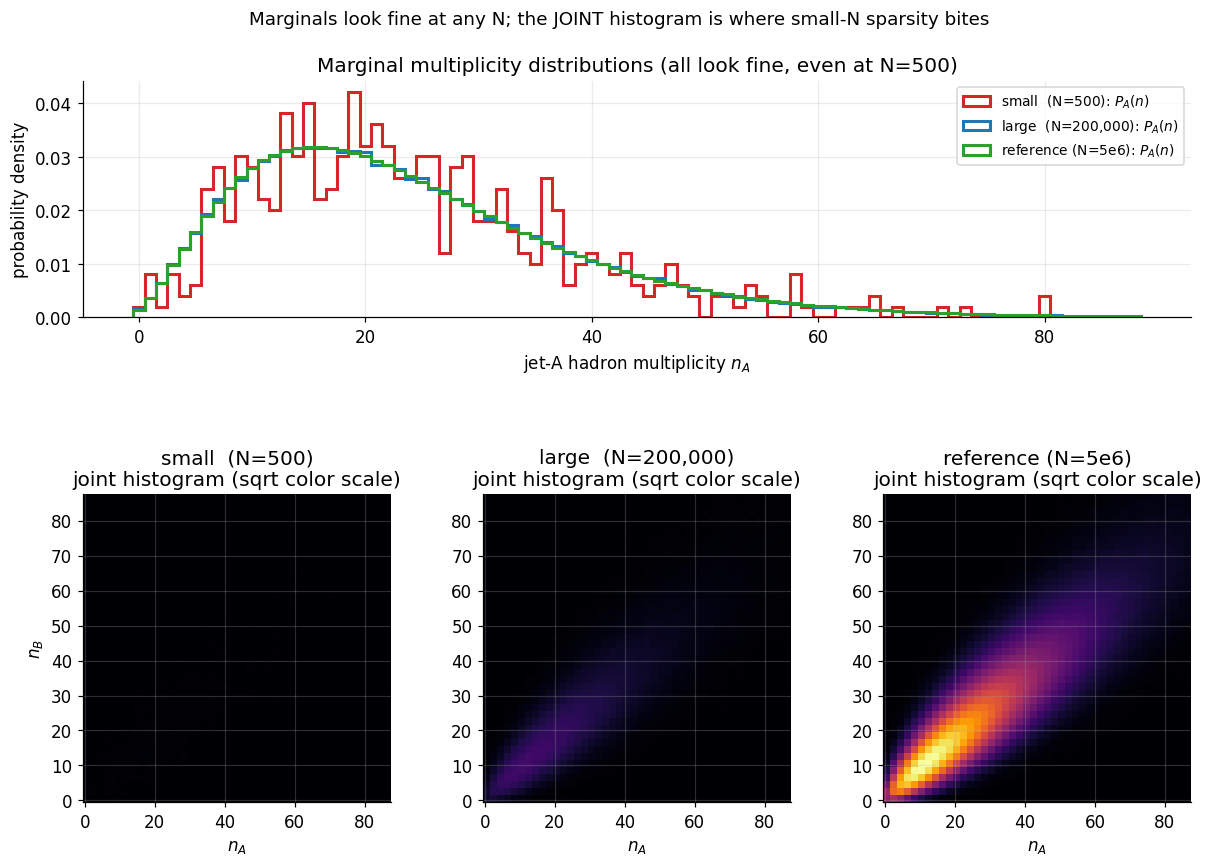
\includegraphics[width=\textwidth]{figs/fig01_marginals_joint.png}
\caption{Marginal multiplicity distributions (top) and 2D joint histograms
(bottom, square-root color scale) for the small, large, and reference
samples. Marginals look consistent at any $N$; the joint histogram is
where small-$N$ sparsity bites.}
\label{fig:marginals-joint}
\end{figure}

\subsection{Bias vs.\ sample size}

Repeating the naive estimate over a range of $N$ (with several repetitions
per $N$ to see the scatter) and plotting $\hat I_{\rm naive}$ against
$1/N$ (Fig.~\ref{fig:bias-vs-N}) shows the systematic downward drift
(bias shrinking) as $N$ grows, converging toward the flat reference line,
and the expected near-linear behavior in $1/N$: the intercept of that line
is a cheap, model-independent estimate of the bias-corrected/true MI. The
extrapolated intercept, $0.9427$ nats, lands reasonably close to the
reference value of $0.7329$ nats.

\begin{figure}[htb]
\centering
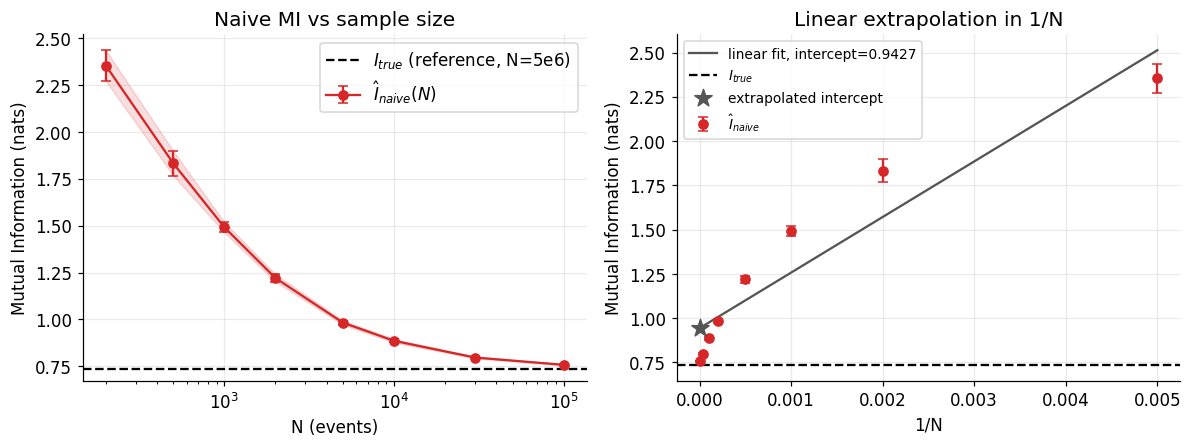
\includegraphics[width=\textwidth]{figs/fig02_bias_vs_N.png}
\caption{Left: naive $\hat I$ vs.\ sample size $N$, converging to the
reference value. Right: the same data plotted against $1/N$, with a linear
extrapolation to $1/N\to0$.}
\label{fig:bias-vs-N}
\end{figure}

% =============================================================================
\section{Corrections: Miller--Madow and shuffle-subtraction}
\label{sec:corrections}
% =============================================================================

\subsection{Miller--Madow correction}

The exact leading-order Miller--Madow correction applies the
$-(K-1)/(2N)$ term to \emph{each} of $S_A,S_B,S_{AB}$ separately and
combines them:
\begin{equation}
\hat I_{MM} = \hat I_{\rm naive} - \frac{(K_{AB}-1)-(K_A-1)-(K_B-1)}{2N}
= \hat I_{\rm naive} - \frac{K_{AB}-K_A-K_B+1}{2N}.
\end{equation}
Crucially, $K_{AB}$ here must be the \emph{actually observed} number of
occupied joint bins, not the product $K_AK_B$: for correlated variables
(our case, by construction) the joint distribution concentrates on a
narrow ridge and $K_{AB}\ll K_AK_B$, so using the product in place of the
observed value wildly overcorrects and can drive $\hat I_{MM}$ negative.

\subsection{Shuffle-subtraction (label-permutation null)}

Randomly permuting the $B$-jet labels relative to the $A$-jet labels
\emph{within the same sample} destroys any true correlation
($I_{\rm true,shuffled}=0$ by construction) while reproducing the same
finite-sample bias. Averaging over many shuffles gives a direct empirical
estimate of the bias to subtract:
\begin{equation}
\hat I_{\rm corrected} = \hat I_{\rm naive} -
\big\langle \hat I_{\rm shuffled}\big\rangle .
\end{equation}
This makes no asymptotic assumption and remains reliable even when
$N\lesssim K_AK_B$, where Miller--Madow starts to break down. It has its
own bias, however: shuffling spreads the joint distribution over
\emph{more} bins than the true correlated data occupies, so the shuffled
surrogate is \emph{more} undersampled than the real data at the same $N$.
Shuffle-subtraction therefore tends to systematically
\textbf{overestimate} the bias and \textbf{overcorrect}, pulling
$\hat I_{\rm corrected}$ below $\Itrue$ when the true correlation is
strong.

\begin{table}[h]
\centering
\caption{Naive, Miller--Madow, and shuffle-corrected $\hat I$ vs.\ $N$.}
\begin{tabular}{rrrrr}
\toprule
$N$ & $\hat I_{\rm naive}$ & $\hat I_{MM}$ & $\hat I_{\rm shuffle}$ & $\Itrue$ (ref.) \\
\midrule
200    & 2.2764 & 2.0889 & 0.0657 & 0.7329 \\
500    & 1.8694 & 1.6014 & 0.1436 & 0.7329 \\
1000   & 1.4271 & 1.1756 & 0.2422 & 0.7329 \\
2000   & 1.1873 & 0.9866 & 0.3809 & 0.7329 \\
5000   & 0.9766 & 0.8539 & 0.5592 & 0.7329 \\
20000  & 0.8259 & 0.7750 & 0.6792 & 0.7329 \\
\bottomrule
\end{tabular}
\end{table}

With the correct Miller--Madow formula (using the observed $K_{AB}$), both
corrections pull the small-$N$ estimates much closer to $\Itrue$ than the
naive value and stay well-behaved (no more diving negative). Neither lands
exactly on $\Itrue$ at very small $N$: Miller--Madow is only a
first-order truncation of the true bias expansion, and shuffle-subtraction
overcorrects when the true correlation is strong, as explained above. Both
effects shrink as $N$ grows.

The shuffle procedure gives more than a bias correction -- the spread of
$\hat I_{\rm shuffled}$ over many permutations \emph{is} the null
distribution for ``$\Itrue=0$'' at that $N$ and binning
(Fig.~\ref{fig:shuffle-null}). Plotting $\hat I_{\rm naive}$ against that
null distribution is a direct visual significance check: at $N=500$ the
null distribution itself is already centered well above zero (pure bias)
and the naive value sits close to or inside this null cloud, so on its own
it would not be significant evidence of correlation, even though the jets
are truly correlated by construction. By $N=20{,}000$ the null has
collapsed toward zero and the naive value clearly separates from it.

\begin{figure}[htb]
\centering
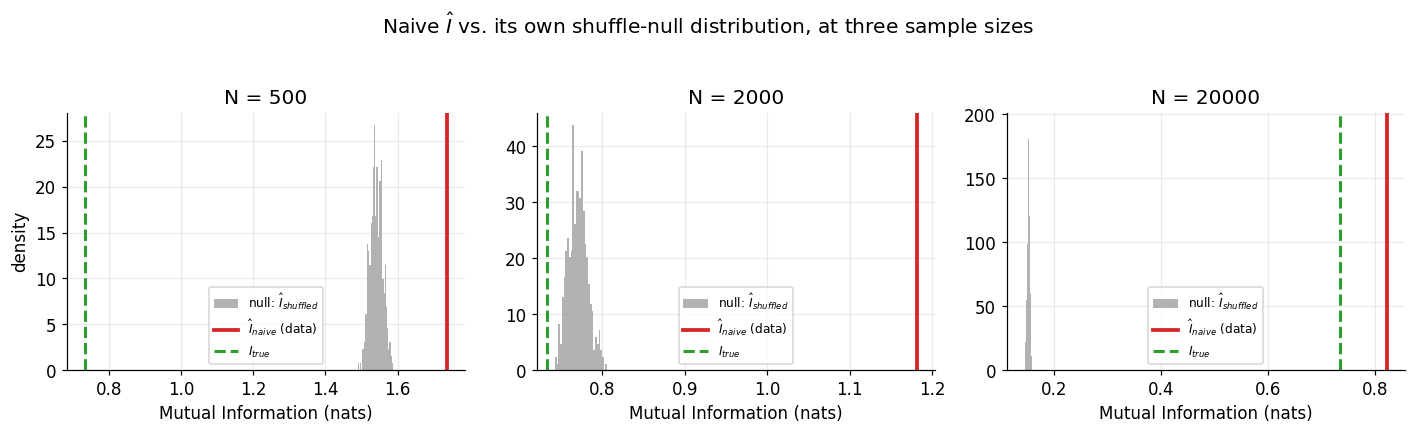
\includegraphics[width=\textwidth]{figs/fig03_shuffle_null.png}
\caption{Naive $\hat I$ (vertical line) against its own shuffle-null
distribution (histogram), at three sample sizes. Dashed line: true value.}
\label{fig:shuffle-null}
\end{figure}

Figure~\ref{fig:naive-vs-corrected} summarizes naive vs.\ corrected MI
across sample sizes, and Fig.~\ref{fig:residuals} plots
$|\hat I - \Itrue|$ on a log-log scale, which is the honest way to compare
convergence rates. Both corrections sit visibly below the naive curve at
fixed $N$; where the corrected residual curves run roughly parallel to the
naive curve rather than dropping faster, that indicates the residual error
is increasingly dominated by sub-leading bias terms that neither method
captures (Miller--Madow: higher-order $1/N^2,\ldots$ terms; shuffle: the
systematic overcorrection discussed above) -- exactly the gap the more
rigorous fix in Sec.~\ref{sec:nsb} is designed to close.

\begin{figure}[htb]
\centering
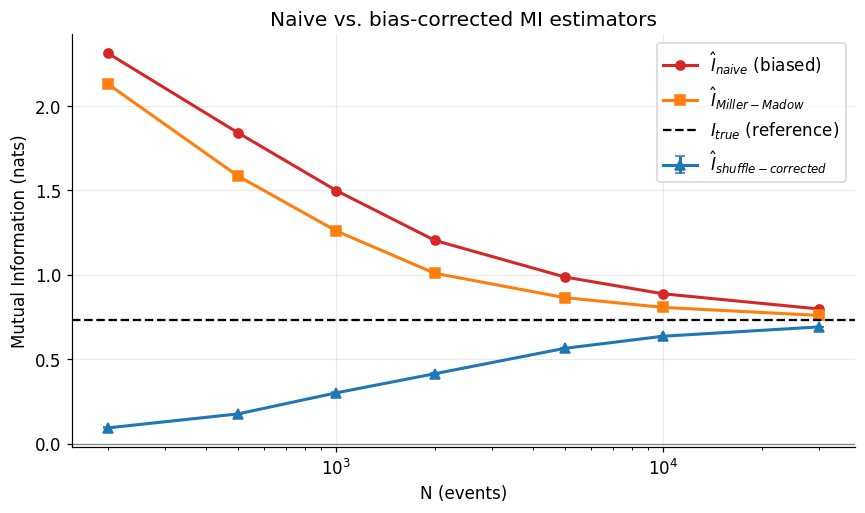
\includegraphics[width=0.75\textwidth]{figs/fig04_naive_vs_corrected.png}
\caption{Naive vs.\ bias-corrected MI estimators across sample sizes.}
\label{fig:naive-vs-corrected}
\end{figure}

\begin{figure}[htb]
\centering
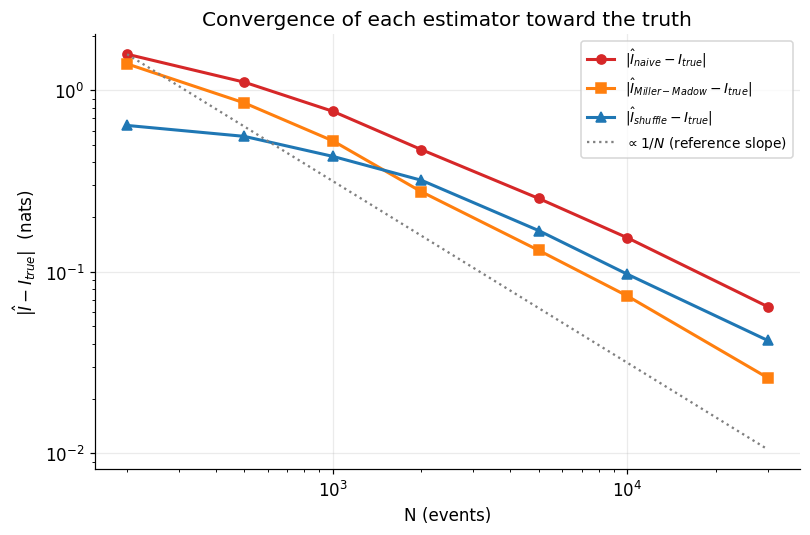
\includegraphics[width=0.75\textwidth]{figs/fig05_residual_convergence.png}
\caption{Convergence of each estimator toward the true value, on a log-log
scale, with a $1/N$ reference slope.}
\label{fig:residuals}
\end{figure}

% =============================================================================
\section{The rigorous fix: NSB Bayesian entropy estimator}
\label{sec:nsb}
% =============================================================================

Both corrections above are still, fundamentally, \textbf{point corrections
derived under a large-$N$ assumption} -- they estimate one number (the
bias) and subtract it. The \textbf{Nemenman--Shafee--Bialek (NSB)}
estimator takes a genuinely different approach: instead of correcting a
biased point estimate, it computes the \textbf{Bayesian posterior mean
entropy} directly, using a prior specifically constructed to avoid
smuggling in any implicit assumption about how spread-out the distribution
is. This is the standard tool for the severely-undersampled regime
($N\lesssim K$) in the neuroscience spike-train MI literature -- precisely
our regime once hadron multiplicities are binned in 2D.

The construction, in four steps:

\begin{enumerate}
\item Put a symmetric Dirichlet prior $P(p\,|\,\beta)\propto\prod_i
p_i^{\beta-1}$ over the $K$ possible bin probabilities. For any fixed
$\beta$, the posterior mean entropy given counts $\{n_i\}$ has a closed
form,
\begin{equation}
\langle S\rangle_{\beta,n} = \psi_0(N+K\beta+1) -
\sum_i \frac{n_i+\beta}{N+K\beta}\,\psi_0(n_i+\beta+1).
\end{equation}

\item \textbf{The catch:} a flat prior on $\beta$ does \emph{not} give a
flat prior on entropy -- for large $K$, $P(S\,|\,\beta)$ is sharply peaked
as a function of $\beta$. Fixing any single $\beta$ (as ordinary
add-one/Laplace/Jeffreys smoothing does) silently assumes an entropy value
before looking at the data.

\item NSB's fix: reweight $\beta$ by the hyperprior that makes the
\emph{induced} prior on $S$ flat -- literally the rate of change of the
prior mean entropy with $\beta$,
\begin{equation}
\rho(\beta) = K\,\psi_1(K\beta+1) - \psi_1(\beta+1).
\end{equation}

\item Average over $\beta$, weighted by both this hyperprior and the
Dirichlet--multinomial evidence $P(n\,|\,\beta)$,
\begin{equation}
\hat S_{\rm NSB} =
\frac{\int_0^\infty d\beta\;\rho(\beta)\,P(n\,|\,\beta)\,\langle
S\rangle_{\beta,n}}
{\int_0^\infty d\beta\;\rho(\beta)\,P(n\,|\,\beta)}.
\end{equation}
\end{enumerate}

This reduces to a tractable 1D numerical integral. We apply it separately
to $S_A,S_B,S_{AB}$ (each needs its own alphabet size $K$: for the joint
distribution, $K_{AB}^{\rm alphabet}=K_A^{\rm alphabet}\times K_B^{\rm
alphabet}$, the full product space of possible outcomes -- not the
observed $K_{AB}$ count from before, since NSB needs to know the size of
the space being integrated over, not how much of it happened to be hit),
then combine: $\hat I_{\rm NSB} = \hat S_A^{\rm NSB}+\hat S_B^{\rm
NSB}-\hat S_{AB}^{\rm NSB}$.

\begin{table}[h]
\centering
\caption{All four MI estimators, head to head.}
\begin{tabular}{rrrrrr}
\toprule
$N$ & $\hat I_{\rm naive}$ & $\hat I_{MM}$ & $\hat I_{\rm shuffle}$ &
$\hat I_{\rm NSB}$ & $\Itrue$ (ref.) \\
\midrule
200   & 2.3511 & 2.1711 & 0.0578 & 0.5098 & 0.7329 \\
500   & 1.7525 & 1.5035 & 0.2137 & 0.6833 & 0.7329 \\
1000  & 1.5071 & 1.2711 & 0.3062 & 0.7369 & 0.7329 \\
2000  & 1.2299 & 1.0367 & 0.4340 & 0.7416 & 0.7329 \\
5000  & 1.0030 & 0.8842 & 0.5807 & 0.7678 & 0.7329 \\
20000 & 0.8222 & 0.7716 & 0.6752 & 0.7411 & 0.7329 \\
\bottomrule
\end{tabular}
\end{table}

NSB tracks $\Itrue$ closely across the entire range, including at
$N=200$ where the naive estimator is off by roughly a factor of three and
Miller--Madow has barely moved. This is the payoff of treating the whole
problem as Bayesian inference over entropy rather than patching a biased
point estimate after the fact. Figure~\ref{fig:nsb-comparison} adds NSB to
the convergence comparison: its residual curve sits visibly below the
other three methods across most of the range, and in particular stays far
more stable at small $N$ -- it doesn't need $N\gg K$ to behave sensibly.

\begin{figure}[htb]
\centering
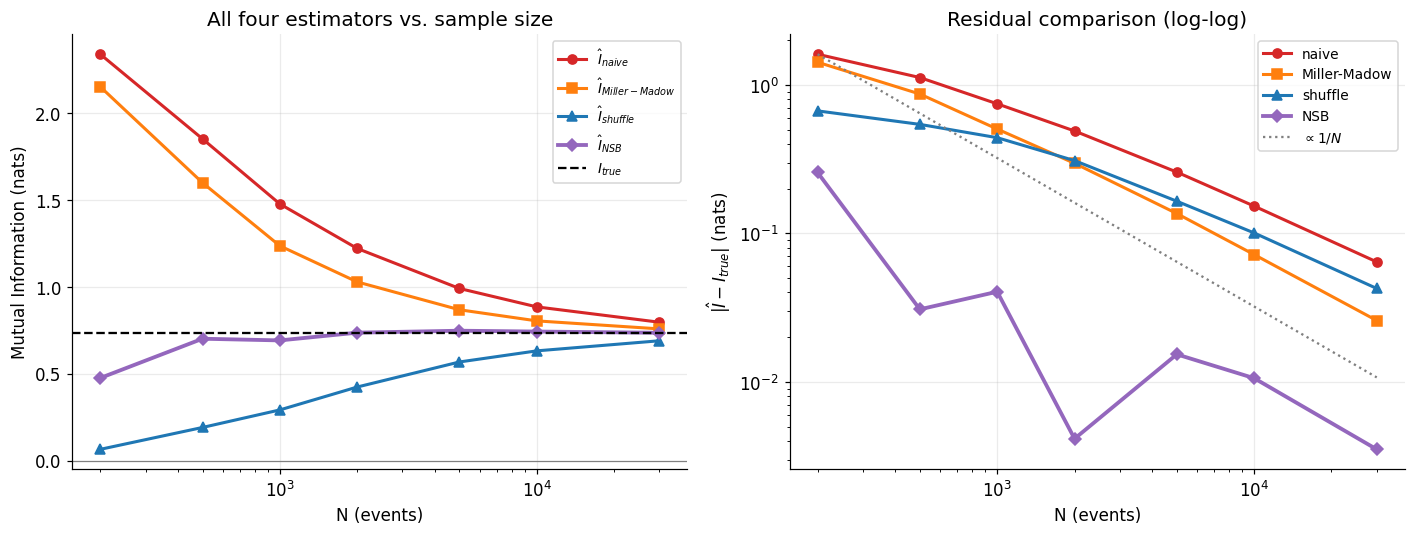
\includegraphics[width=\textwidth]{figs/fig06_nsb_comparison.png}
\caption{Left: all four estimators vs.\ sample size. Right: residual
comparison on a log-log scale, with a $1/N$ reference slope.}
\label{fig:nsb-comparison}
\end{figure}

\paragraph{Practical notes for the real STAR dijet data.}
\begin{itemize}
\item The alphabet size $K$ (for each marginal, and $K_A\times K_B$ for
the joint) needs to be fixed \emph{before} looking at the data -- pick a
generous fixed upper bound on plausible hadron multiplicity per jet
(e.g.\ from detector acceptance / kinematic limits), not the observed
range, or a data-dependent bias is reintroduced through the back door.
\item NSB is somewhat more expensive per call than MM or
shuffle-subtraction (a 1D numerical integral instead of a closed-form
correction or a handful of permutations), but it remains a fraction of a
second per event sample -- entirely practical for a real analysis,
including a full jackknife or bootstrap for uncertainty quantification.
\item The same estimator applies directly to $\SBA=S_{AB}-S_A$ -- swap in
the NSB entropies there instead of the naive/MM/shuffle versions before
making any negative-conditional-entropy (quantum) claim, as done next.
\end{itemize}

% =============================================================================
\section{Putting it together: quantum-signal detection sensitivity}
\label{sec:sensitivity}
% =============================================================================

Section~\ref{sec:observable} established $\SBA=S_{AB}-S_A$ as the correct,
computable witness (provably $\geq0$ classically), and
Secs.~\ref{sec:bias}--\ref{sec:nsb} established that NSB is the
best-behaved bias-corrected estimator, especially at small $N$. Here we
combine both: since our toy model is itself purely classical, its true
$\SBA$ is a known, solidly positive number ($\SBA_{\rm true}=3.1524$
nats) -- exactly the right sandbox to measure the \textbf{statistical
noise floor} of the NSB estimator against a known ground truth, and turn
that into a quantitative statement about how large a genuine quantum
excess would need to be, at a given event count, to be distinguishable
from this noise floor.

\textbf{Design:} for a grid of $N$, we draw many independent samples from
the same generative model, compute $\hat S(B|A)_{\rm NSB}$ for each, and
take the spread over draws as the estimator's sampling uncertainty
$\sigma_{\rm NSB}(N)$ at that statistics. A hypothetical genuine quantum
excess of magnitude $\Delta$ is then detectable at $z$ standard
deviations once
\begin{equation}
\Delta \;>\; z\,\sigma_{\rm NSB}(N).
\end{equation}
Equivalently, the \textbf{minimum detectable quantum signal} at a chosen
confidence level ($z=3$, a common ``solid evidence'' threshold, used
below) is $\Delta_{\rm min}(N)=z\,\sigma_{\rm NSB}(N)$. In a real analysis
with one actual dataset -- not a synthetic model with known truth --
$\sigma_{\rm NSB}(N)$ would be estimated directly from that dataset via
bootstrap or jackknife resampling, rather than from independent Monte
Carlo replicates as done here for demonstration.

Figure~\ref{fig:noise-floor} shows the NSB (and, for comparison, naive and
Miller--Madow) estimates of $\SBA$ vs.\ $N$, together with their
sampling standard deviation. NSB has both the smallest bias (its mean
tracks $\SBA_{\rm true}$ most closely, especially at small $N$) and a
noise floor that shrinks cleanly with $N$, following the expected
$1/\sqrt{N}$ statistical scaling.

\begin{figure}[htb]
\centering
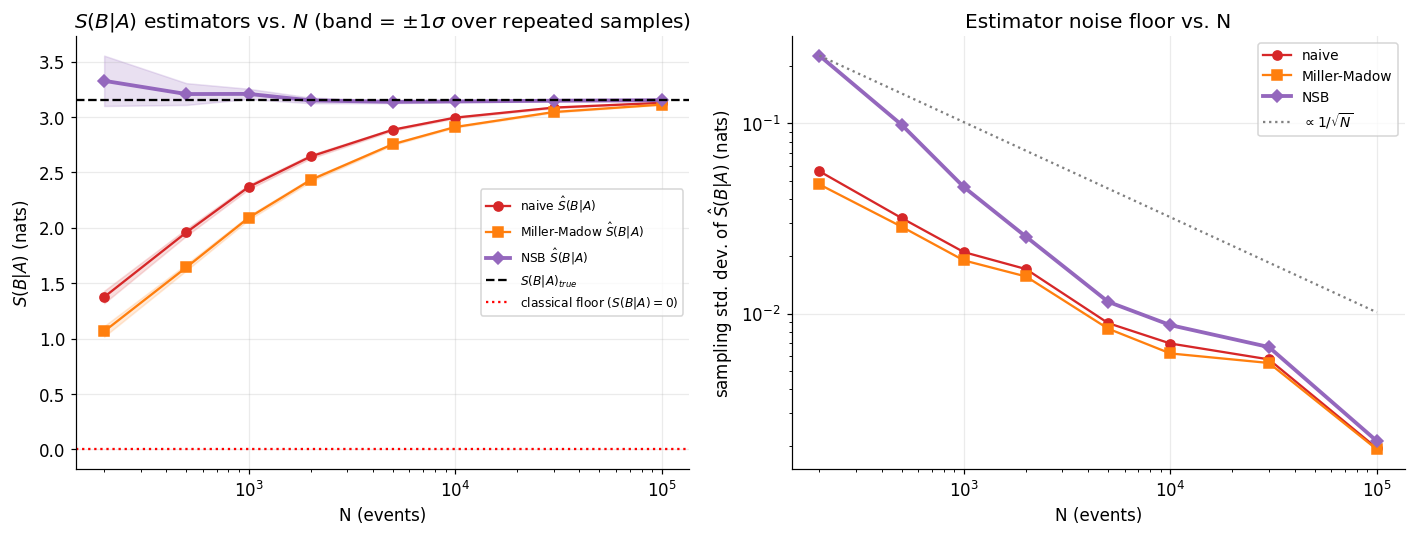
\includegraphics[width=\textwidth]{figs/fig07_sba_noise_floor.png}
\caption{Left: $\SBA$ estimators vs.\ $N$ (bands: $\pm1\sigma$ over
repeated samples). Right: sampling standard deviation of each estimator
vs.\ $N$, with a $1/\sqrt{N}$ reference slope.}
\label{fig:noise-floor}
\end{figure}

Converting the NSB noise floor into a minimum-detectable-signal curve
(Fig.~\ref{fig:detection-sensitivity}) and fitting a power law gives a
direct, quantitative answer to ``how big must a quantum signal be, at a
given statistics, to be believable'':

\begin{table}[h]
\centering
\caption{Minimum event count $N$ needed for a $3\sigma$ detection of a
hypothetical quantum-correlation excess of the given magnitude, from the
fitted $\Delta_{\rm min}(N)\propto N^{-0.72}$ power law.}
\begin{tabular}{rr}
\toprule
Assumed $|\SBA_{\rm quantum}|$ (nats) & $N$ needed for $3\sigma$ detection \\
\midrule
0.500 & 201 \\
0.200 & 722 \\
0.100 & 1{,}899 \\
0.050 & 4{,}995 \\
0.020 & 17{,}934 \\
0.010 & 47{,}164 \\
\bottomrule
\end{tabular}
\end{table}

\begin{figure}[htb]
\centering
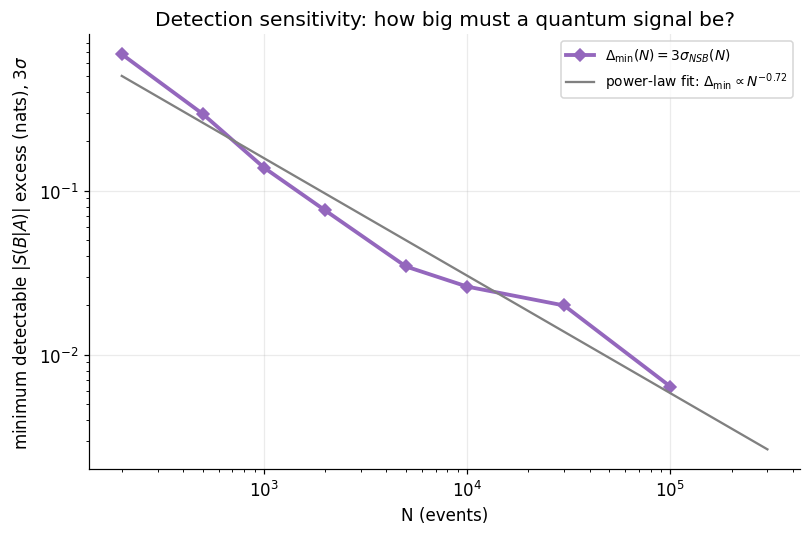
\includegraphics[width=0.75\textwidth]{figs/fig08_detection_sensitivity.png}
\caption{Minimum detectable $|\SBA|$ excess at $3\sigma$, vs.\ event
count $N$, with a power-law fit for interpolation/extrapolation.}
\label{fig:detection-sensitivity}
\end{figure}

\paragraph{Caveats to carry into the real analysis.}
\begin{itemize}
\item $\sigma_{\rm NSB}(N)$ here is measured \emph{at the true classical
value} ($\SBA_{\rm true}\approx$ a few nats for our toy correlation
strength), not at the boundary $\SBA=0$. Entropy-estimator variance
depends on the shape of the underlying distribution, not just $N$, so the
true noise floor near a genuinely small or slightly-negative $\SBA$ could
differ somewhat from this estimate. For the real STAR data, this bootstrap
procedure should be re-run centered on the actual observed operating point
(via jackknife/bootstrap on the real dataset itself), rather than trusting
this toy-model number directly.
\item This procedure characterizes sensitivity to a violation of the
classical conditional-entropy bound using multiplicity data alone
(Sec.~\ref{sec:observable}). It is not a substitute for an actual quantum
witness such as a Bell/CHSH inequality on the $\Lambda\bar\Lambda$ spin
observables, which remains the model-independent way to certify
entanglement rather than merely rule out one particular classical
description.
\end{itemize}

% =============================================================================
\section{Summary and recommendations from the toy Monte Carlo study}
% =============================================================================

\begin{enumerate}

\item \textbf{The correct witness} is $\SBA=S_{AB}-S_A$ (and $S(A|B)$,
check both directions), which must be $\geq0$ for any classical
distribution. Genuine quantum discord (Ollivier--Zurek) cannot be
computed from hadron-count histograms alone -- any classical joint
distribution trivially gives discord $=0$; it would require actual
quantum-state tomography (e.g.\ the $\Lambda\bar\Lambda$
spin-density-matrix channel).

\item \textbf{The naive plug-in MI estimator is always biased upward},
with leading term $\approx(K_{AB}-K_A-K_B+1)/(2N)$. Coarser binning or
fewer events both make it worse -- comparing different STAR running
periods, luminosities, or binning choices will report different central
MI values from what should be the same physics, purely from this effect.

\item \textbf{Miller--Madow} (done correctly, using the observed
$K_{AB}$, not the product $K_AK_B$) and \textbf{shuffle-subtraction} both
substantially reduce this bias and stay well-behaved, but neither is exact
at small $N$: Miller--Madow is a first-order truncation;
shuffle-subtraction tends to systematically overcorrect when the true
correlation is strong.

\item \textbf{NSB} is the recommended estimator for the real analysis: a
Bayesian posterior-mean entropy built on a prior specifically constructed
to be uninformative about entropy itself. It tracks the truth closely
across the entire tested $N$ range, including deep in the
severely-undersampled regime where the other methods struggle, at a
modest computational cost.

\item \textbf{Before claiming any quantum-correlation excess}, bias-correct
with NSB and compare against the estimator's own sampling noise floor at
that $N$ (bootstrapped from the real dataset via jackknife/bootstrap, not
assumed from this toy model). Section~\ref{sec:sensitivity} works this out
quantitatively: the NSB noise floor shrinks $\propto 1/\sqrt{N}$, giving a
concrete minimum-detectable-signal curve
$\Delta_{\rm min}(N)=z\,\sigma_{\rm NSB}(N)$ -- a direct, quotable answer
to ``how big must a genuine quantum excess be, at a given event count, to
be distinguishable from finite-sample bias and noise.''

\item \textbf{This entire procedure only tests a violation of the
classical conditional-entropy bound.} It is a necessary check before any
stronger quantum claim, but is not itself a model-independent entanglement
certification -- that role is played by the Bell/CHSH-type inequality on
spin observables in the parallel $\Lambda\bar\Lambda$ program.

\end{enumerate}

% =============================================================================
\section{Validation on PYTHIA~8 Monte Carlo simulation}
\label{sec:pythia}
% =============================================================================

The toy model of Secs.~\ref{sec:toymc}--\ref{sec:nsb} demonstrates that the
estimator pipeline behaves correctly on data with a known, simple
generative structure. The natural next step is to check the same pipeline
on a full QCD event generator, where hadron multiplicities arise from
parton showering, hadronization, and (optionally) the underlying event --
none of which was built into the toy model by hand. We generated
back-to-back charged-jet dijets with PYTHIA~8 (Monash 2013 tune,
anti-$k_T$ jets, $R=0.4$, charged final-state particles only, matching a
STAR-TPC-like charged-jet definition) and applied the identical naive/
Miller--Madow/shuffle/NSB pipeline, unmodified, to the generator output.

This particular validation run used LHC-like kinematics
($\sqrt{s}=14$~TeV rather than the $\sqrt{s}=200$~GeV RHIC energy that
motivates the eventual STAR measurement) specifically \emph{because} of
its much wider accessible jet-$p_T$ range: as discussed below
(Sec.~\ref{sec:pythia-ptdep}), the multiplicity-vs-$p_T$ correlation
predicted by QCD is intrinsically a slow, logarithmic effect, and a wide
dynamic range makes it far easier to confirm the pipeline is tracking real
physics rather than an artifact of a narrow kinematic window. The $200$~GeV
run for the actual STAR measurement is a separate, ongoing exercise (see
Sec.~\ref{sec:conclusions}); everything in this section is a
\emph{methods validation}, not a physics result.

\subsection{Multiplicity and $p_T$ distributions}

Figure~\ref{fig:py-mult-dist} shows the charged-multiplicity distributions
for the leading and subleading jets, overlaid with a method-of-moments
Negative-Binomial fit (as in Sec.~\ref{sec:toymc}). Both jets show genuine
overdispersion relative to Poisson (var/mean $=1.55$ for the leading jet,
$1.29$ for the subleading jet), qualitatively consistent with -- though
not identical in shape to -- the NBD-like multiplicity distributions
assumed in the toy model. This is a useful cross-check in its own right:
the toy model's central structural assumption (NBD-shaped marginals) is
not merely a convenient fiction, but a reasonable approximation to what a
full QCD generator actually produces.

\begin{figure}[htb]
\centering
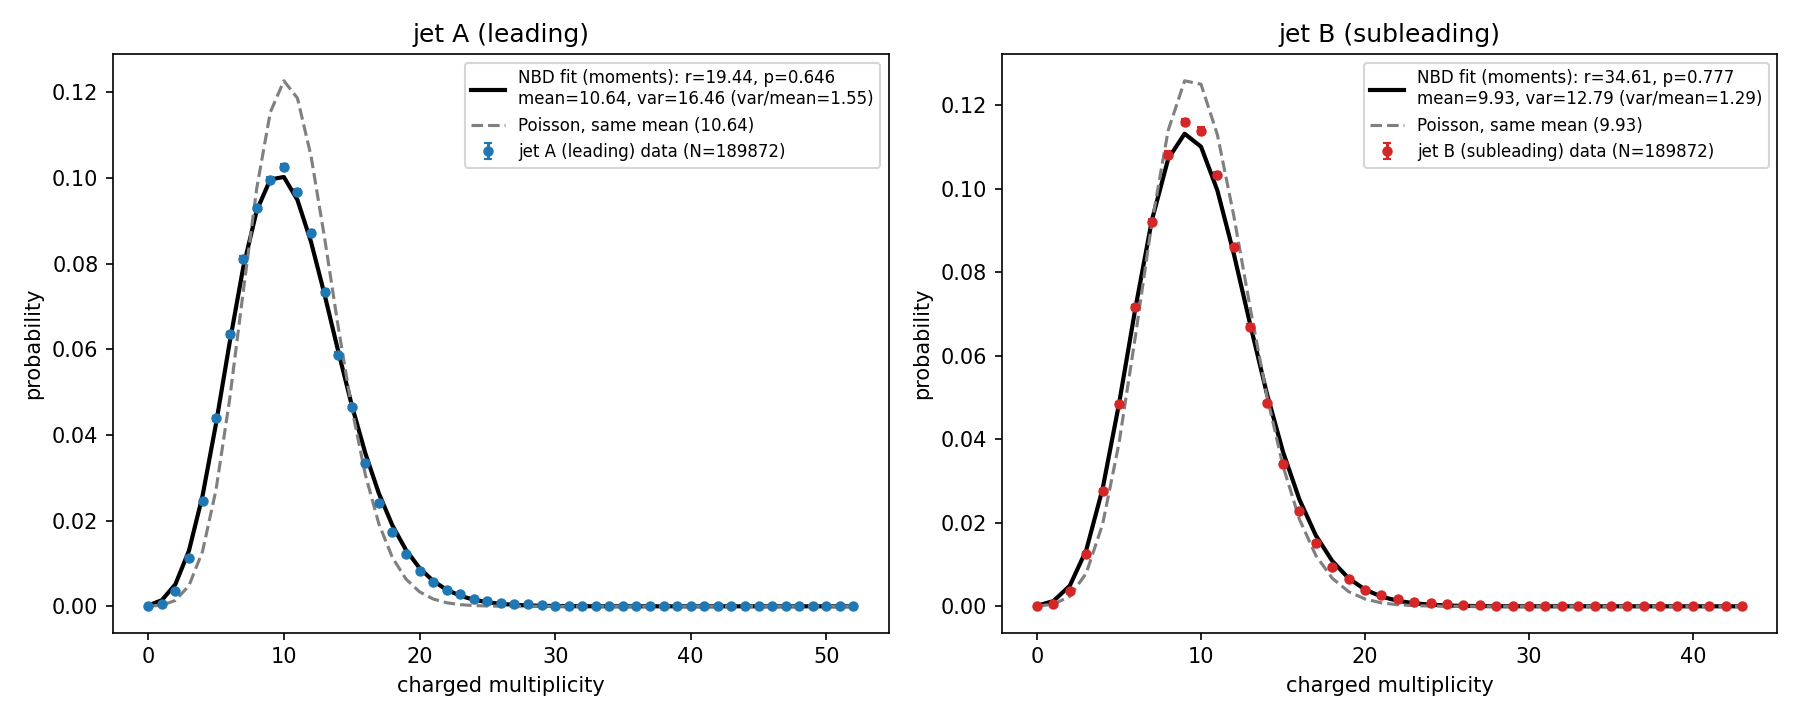
\includegraphics[width=\textwidth]{figs/dijet_entropy_result_truth_multiplicity_dists.png}
\caption{PYTHIA~8: charged-multiplicity distributions for the leading
(left) and subleading (right) jet, with NBD and same-mean Poisson overlay
(cf.\ the toy-model version, Sec.~\ref{sec:toymc}).}
\label{fig:py-mult-dist}
\end{figure}

Figure~\ref{fig:py-joint-mult} shows the corresponding joint distribution:
36.9\% of the $53\times44$ grid is occupied ($K_{AB}=861$) at
$N\approx1.9\times10^5$ events -- a moderately, not severely, undersampled
regime, comparable to the middle of the range explored in the toy study.
Figure~\ref{fig:py-pt-dist} shows the (steeply falling, as expected for a
QCD jet spectrum) leading- and subleading-jet $p_T$ distributions, and
Fig.~\ref{fig:py-joint-pt} their joint distribution -- the latter makes
visually clear why quantile (rather than fixed-width) $p_T$ binning is
necessary for the differential measurements below: the bulk of events sit
in a narrow low-$p_T$ band, with a long, sparse tail.

\begin{figure}[htb]
\centering
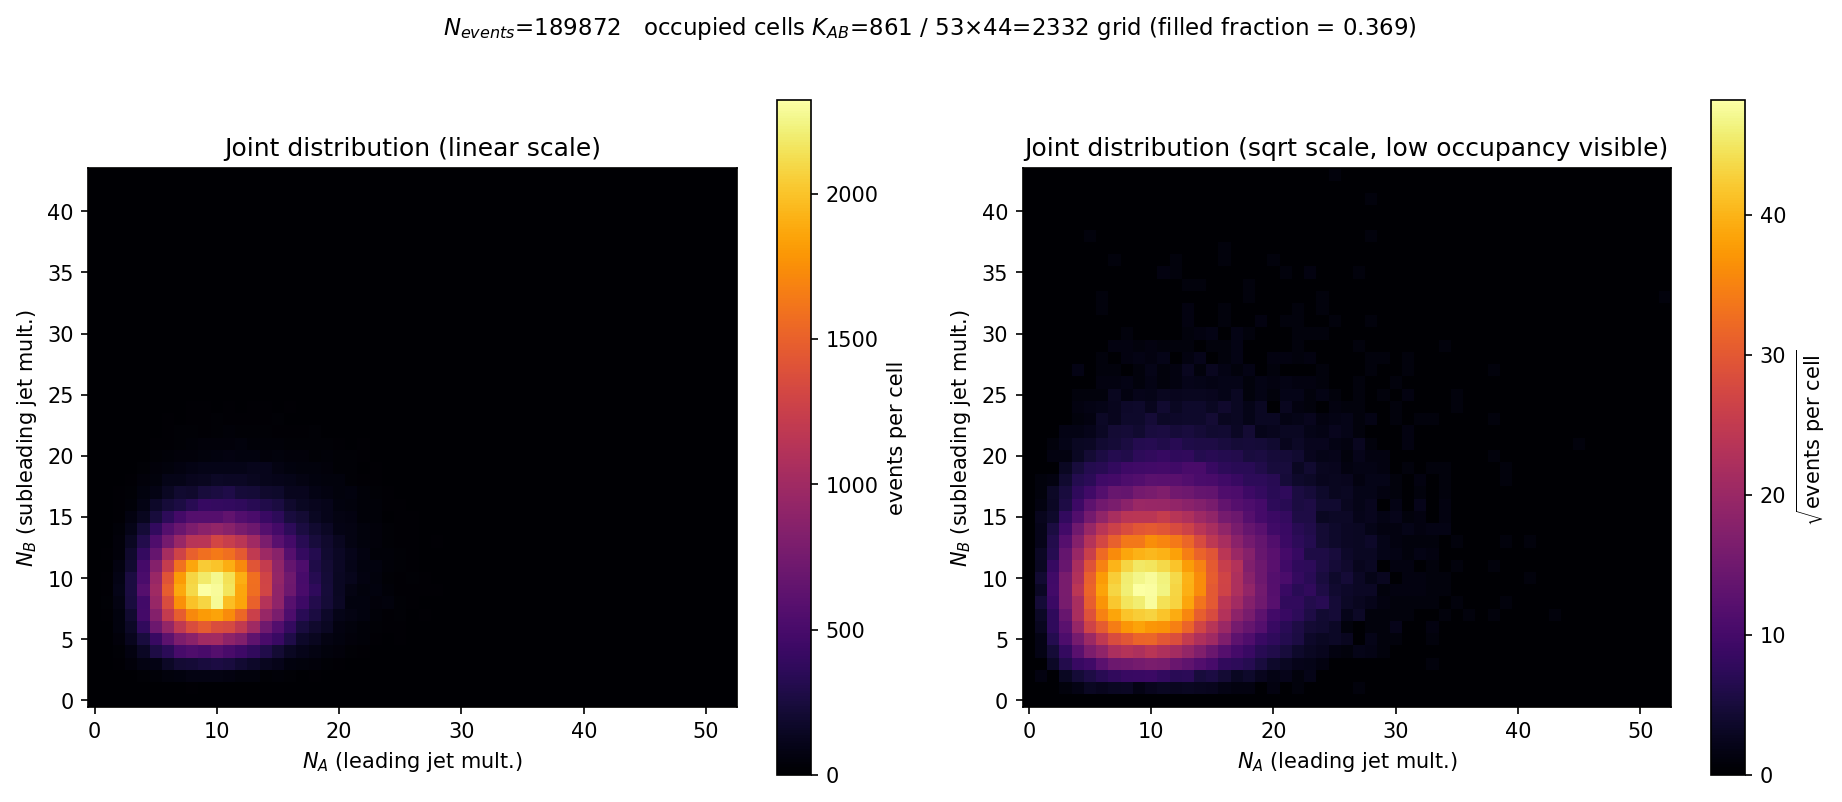
\includegraphics[width=0.85\textwidth]{figs/dijet_entropy_result_truth_joint_multiplicity_dist.png}
\caption{PYTHIA~8: joint charged-multiplicity distribution, linear and
sqrt color scale (cf.\ Fig.~\ref{fig:marginals-joint}).}
\label{fig:py-joint-mult}
\end{figure}

\begin{figure}[htb]
\centering
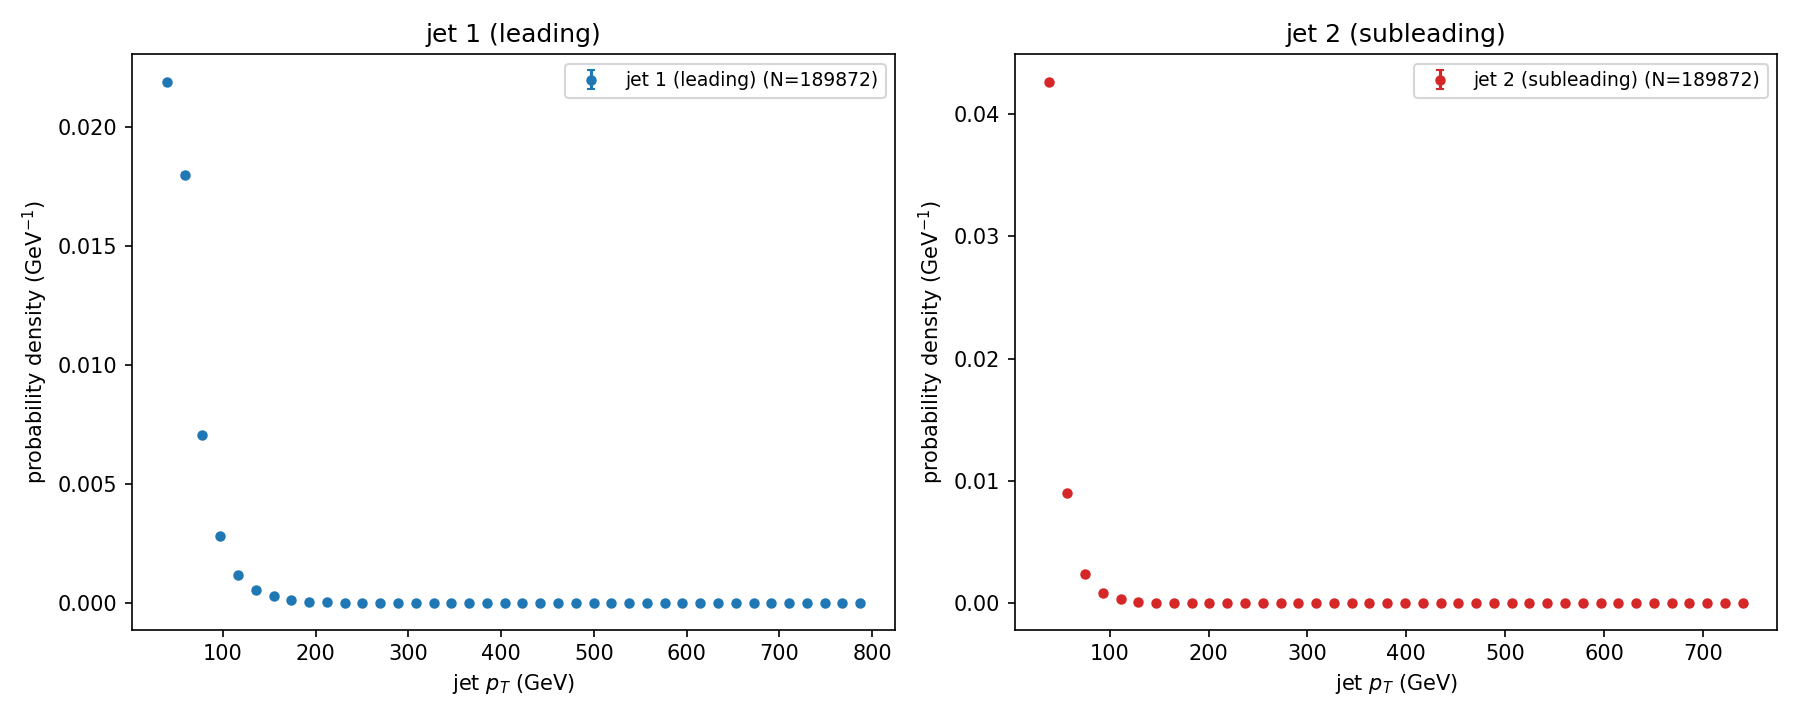
\includegraphics[width=\textwidth]{figs/dijet_entropy_result_truth_pt_dists.png}
\caption{PYTHIA~8: leading- and subleading-jet $p_T$ distributions.}
\label{fig:py-pt-dist}
\end{figure}

\begin{figure}[htb]
\centering
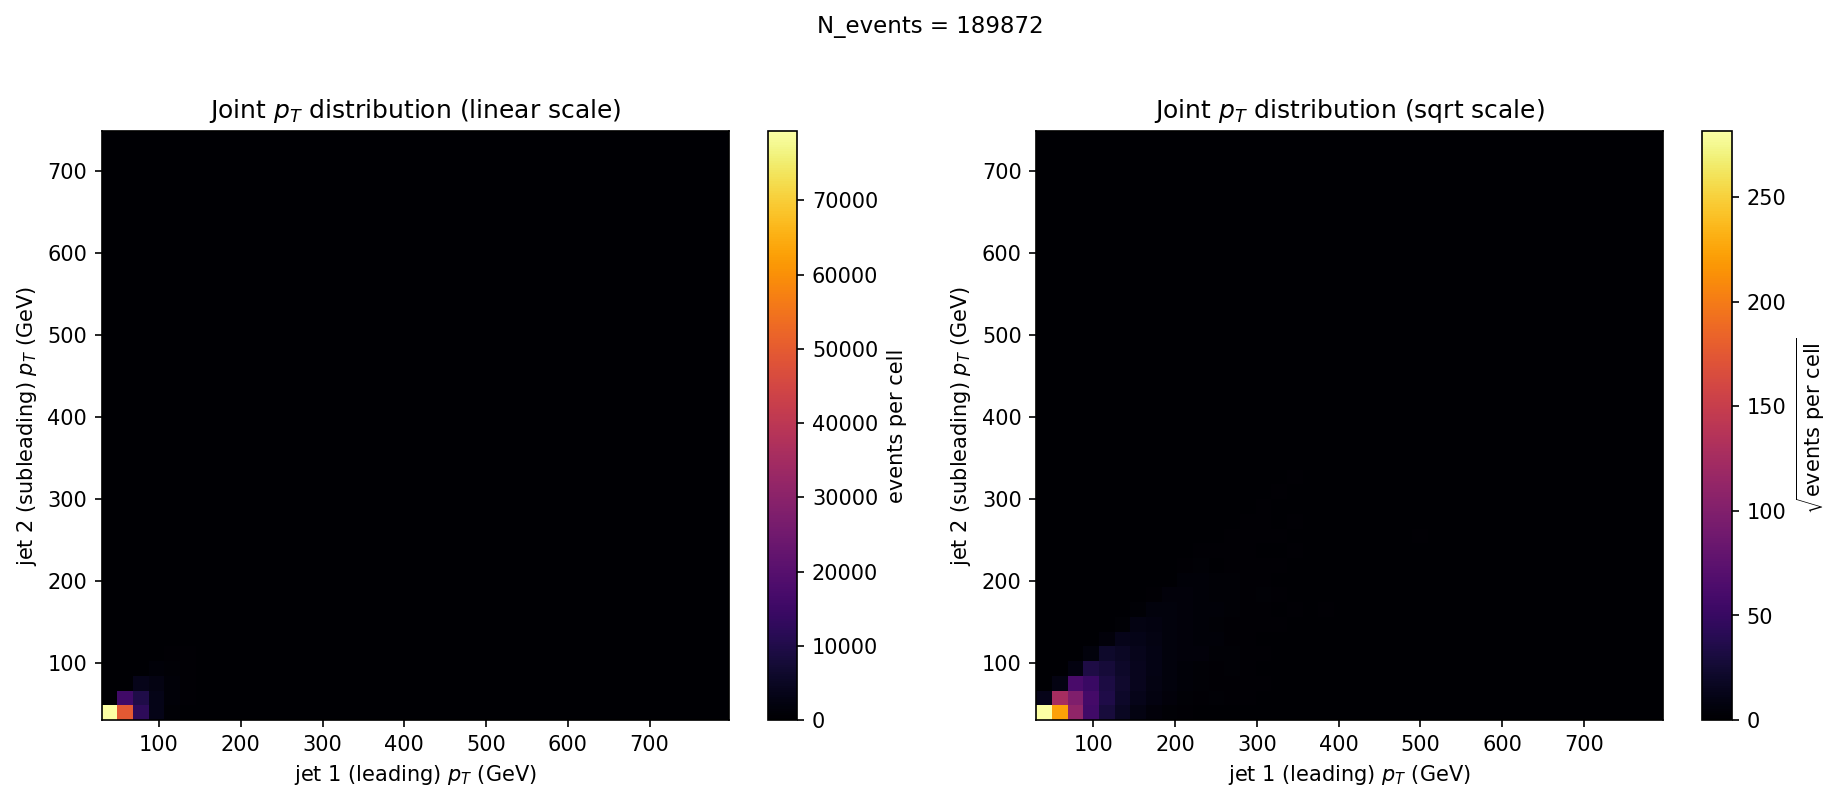
\includegraphics[width=0.85\textwidth]{figs/dijet_entropy_result_truth_joint_pt_dist.png}
\caption{PYTHIA~8: joint leading/subleading jet $p_T$ distribution,
linear and sqrt color scale.}
\label{fig:py-joint-pt}
\end{figure}

\subsection{The multiplicity--$p_T$ correlation}
\label{sec:pythia-ptdep}

A basic physical expectation -- confirmed experimentally (e.g.\ ALICE,
arXiv:2311.13322: ``the mean charged-particle multiplicity inside the
leading jet cone rises monotonically with increasing jet $p_T$'') -- is
that higher-$p_T$ jets should carry higher charged multiplicity, via
additional phase space for parton radiation before hadronization. This
growth is predicted by QCD coherent-branching (MLLA) arguments to be slow
and roughly \emph{logarithmic} in $p_T$, not linear, which matters
directly for how easy the effect is to see over a limited kinematic range
(as it was, initially, in an earlier $200$~GeV validation attempt with a
narrower accessible $p_T$ window).

Figure~\ref{fig:py-mult-vs-pt} shows the raw, unbinned-by-any-entropy-
machinery profile of mean charged multiplicity vs.\ jet $p_T$, together
with a weighted fit of the MLLA-motivated form $\langle N\rangle = a +
b\ln p_T$. The fitted slope is highly significant for both jets ($b =
3.77\pm0.05$, $83\sigma$, leading jet; $b=4.71\pm0.07$, $66\sigma$,
subleading jet) -- direct, quantitative confirmation that PYTHIA~8
reproduces the expected QCD multiplicity-growth pattern, and that the
analysis pipeline correctly recovers it from generator output with no
prior assumption beyond bin means and standard errors.

\begin{figure}[htb]
\centering
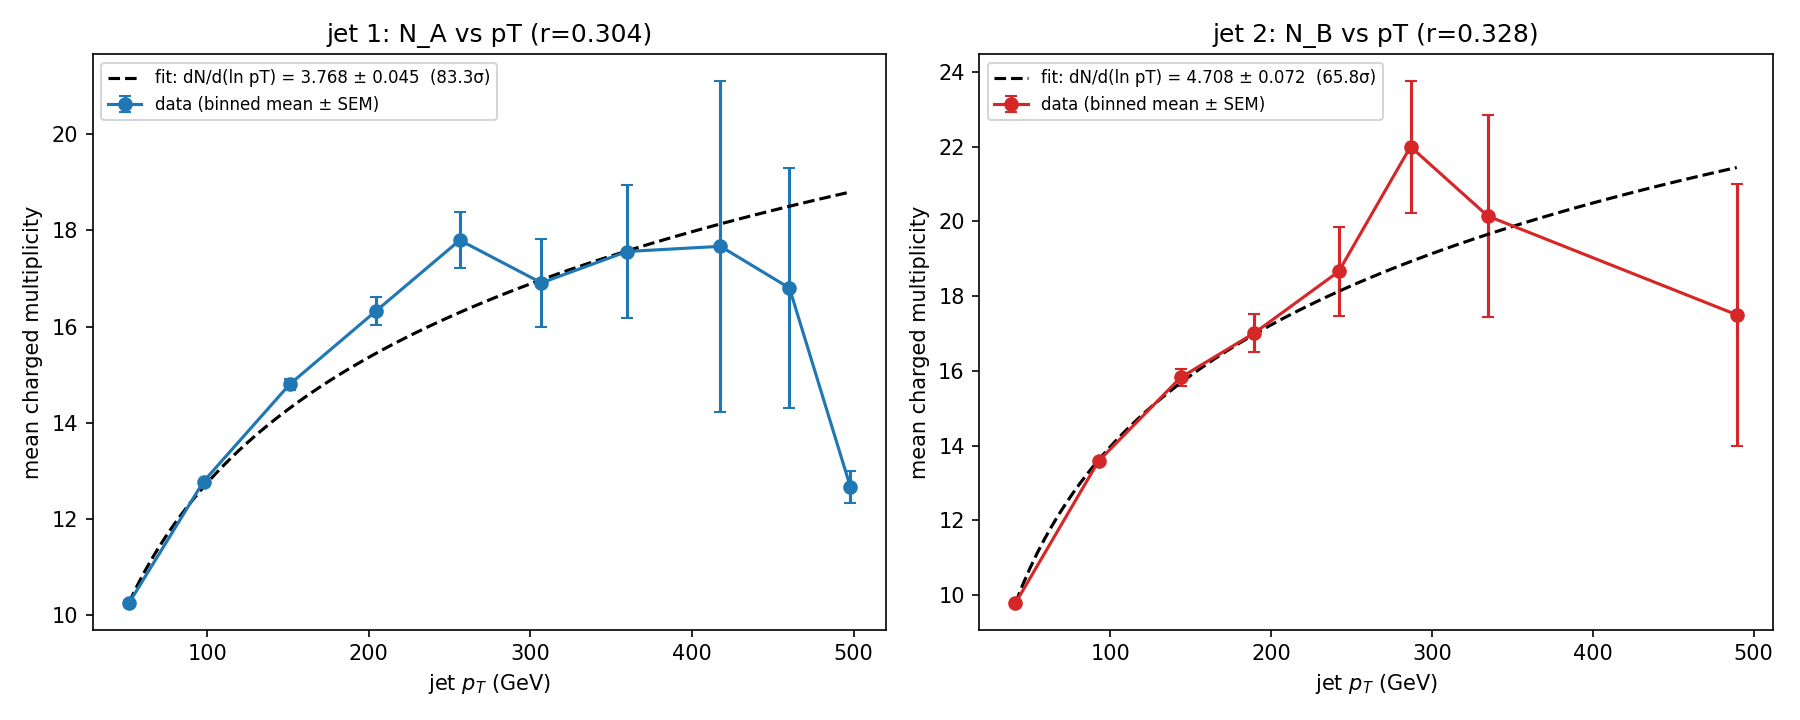
\includegraphics[width=\textwidth]{figs/dijet_entropy_result_truth_mult_vs_pt_profile.png}
\caption{PYTHIA~8: raw mean charged multiplicity vs.\ jet $p_T$ (binned
mean $\pm$ SEM), with a weighted fit to $\langle N\rangle=a+b\ln p_T$.
Both slopes are significant at $>60\sigma$.}
\label{fig:py-mult-vs-pt}
\end{figure}

\subsection{Finite-sample bias, reproduced on generator output}

Figure~\ref{fig:py-bias-scan} repeats the toy study's core diagnostic
(Sec.~\ref{sec:toymc}) directly on subsamples of the real PYTHIA~8 output:
the naive $\hat I$ falls from $\approx0.66$~nats at $N=200$ down toward
the full-sample NSB value ($\approx0.009$~nats) as $N$ grows to
$\approx1.9\times10^5$ -- the same qualitative bias curve seen throughout
Sec.~\ref{sec:toymc}, now confirmed on a dataset the toy model was never
built to resemble. This is a meaningful cross-check: the bias mechanism
identified analytically (Sec.~\ref{sec:bias}) and demonstrated on a
synthetic Gamma-Poisson model is not an artifact of that specific
generative structure -- it appears with the same shape on genuine QCD
Monte Carlo output.

\begin{figure}[htb]
\centering

\includegraphics[width=0.8\textwidth]{figs/dijet_entropy_result_truth_bias_scan.png}
\caption{PYTHIA~8: naive $\hat I$ vs.\ subsample size $N$, real generator
output (cf.\ the toy-model version, Fig.~\ref{fig:bias-vs-N}).}
\label{fig:py-bias-scan}
\end{figure}

\subsection{Point estimates on the full sample}

Figure~\ref{fig:py-summary} shows all four estimators on the full sample
($N\approx1.9\times10^5$): naive ($0.0112\pm0.0004$), Miller--Madow
($0.0092\pm0.0004$), shuffle-corrected ($0.0084\pm0.0003$), and NSB
($0.0085\pm0.0004$~nats) -- naive sits visibly above the other three, as
expected from the bias mechanism above, while Miller--Madow/shuffle/NSB
agree closely with each other, consistent with all three having converged
toward the true value at this statistics (matching the closure seen among
independently-biased estimators at large $N$ in the toy study,
Sec.~\ref{sec:toymc}). The conditional entropy $\SBA=2.65$~nats sits far
above the classical floor, with no indication of a quantum violation --
expected and unsurprising, since PYTHIA~8 is itself a classical
event-by-event simulator with no entanglement built into its hadronization
model. This measurement is a validation of the estimator machinery, not a
physics claim; the analogous measurement on real detector data is where a
genuine quantum question would be asked.

\begin{figure}[htb]
\centering
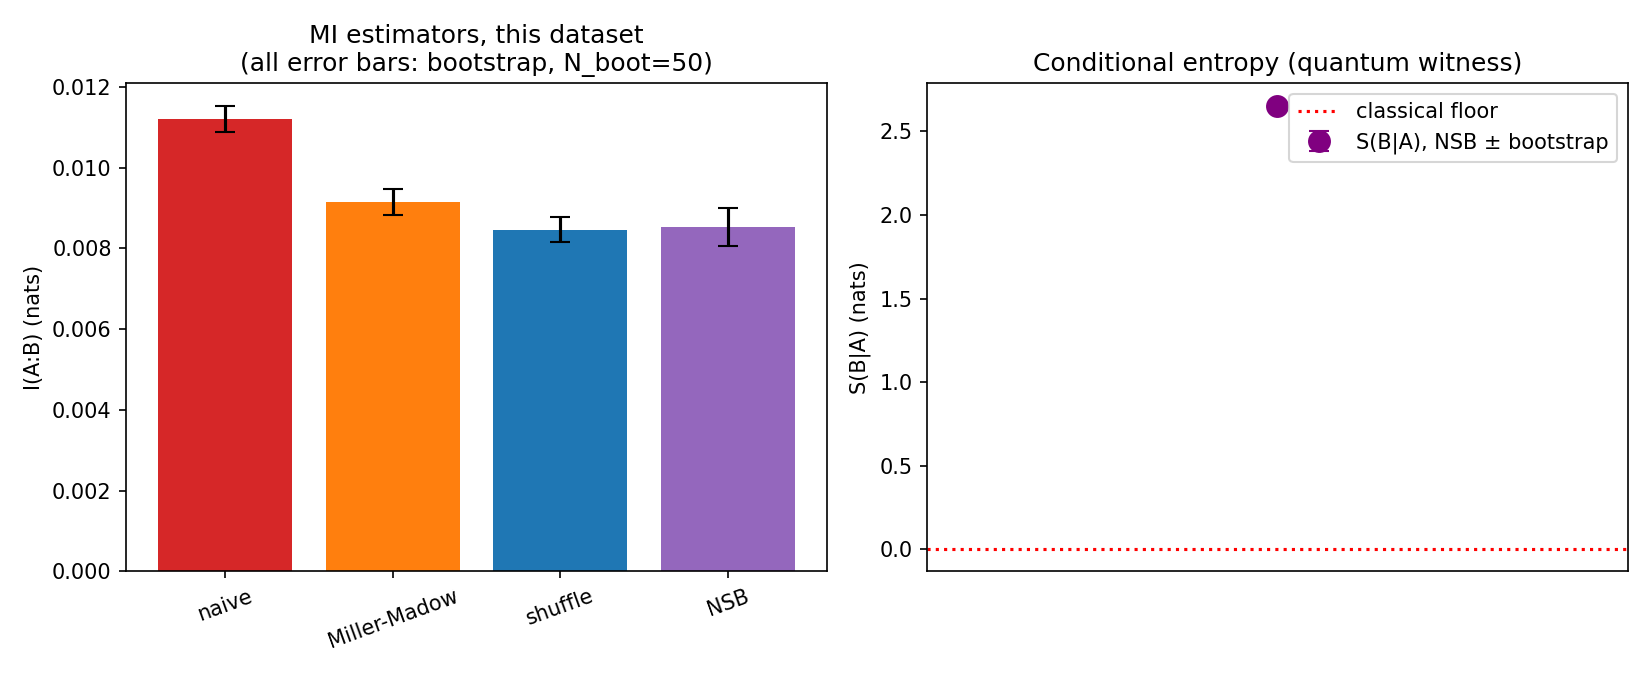
\includegraphics[width=\textwidth]{figs/dijet_entropy_result_truth_summary.png}
\caption{PYTHIA~8: all four MI estimators (left) and $\SBA$ (right) on
the full sample, bootstrap error bars.}
\label{fig:py-summary}
\end{figure}

\subsection{Differential measurement vs.\ jet $p_T$}

Figures~\ref{fig:py-entropy-pt}--\ref{fig:py-sba-pt} show $S_A,S_B,S_{AB}$,
$I(A{:}B)$, and $\SBA$ (NSB) in quantile bins of leading-jet $p_T$. All
three entropies rise smoothly with $p_T$ (Fig.~\ref{fig:py-entropy-pt}),
directly reflecting the multiplicity growth of Sec.~\ref{sec:pythia-ptdep}.
$I(A{:}B)$ (Fig.~\ref{fig:py-mi-pt}) also rises with $p_T$, modestly at
low-to-mid $p_T$ and more sharply in the highest (widest, most
statistics-limited) bin; $\SBA$ (Fig.~\ref{fig:py-sba-pt}) stays solidly
positive and rising throughout, consistent with a classical description at
every $p_T$ probed.

\begin{figure}[htb]
\centering
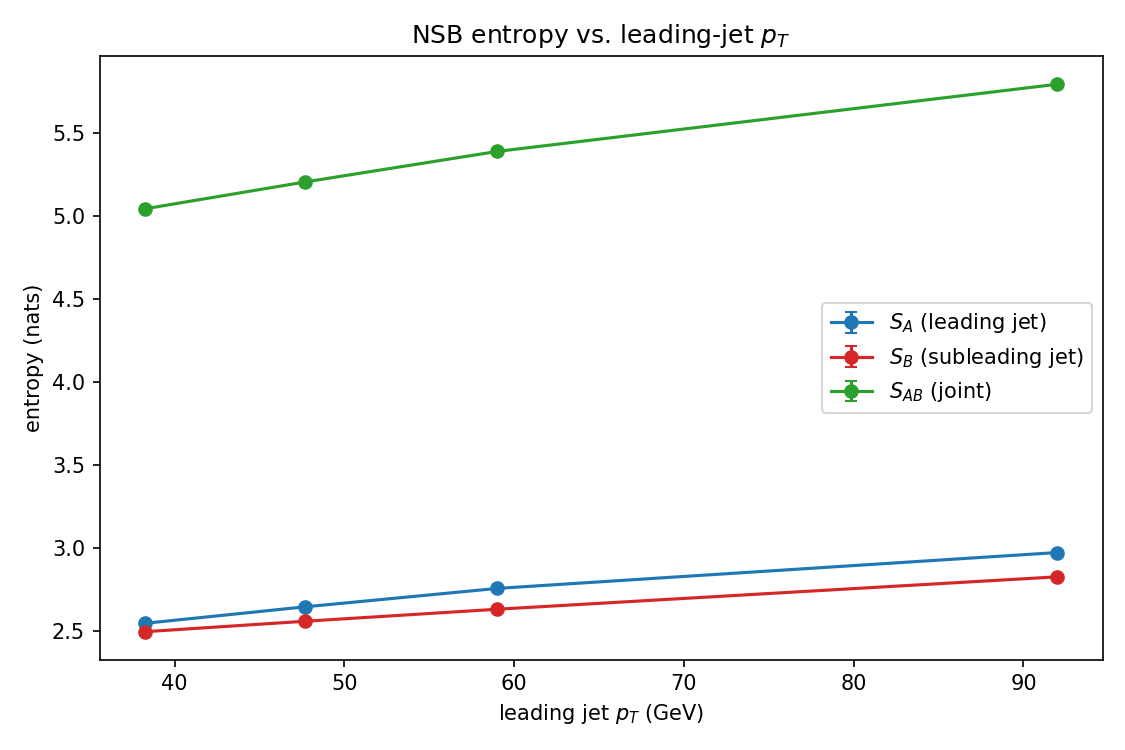
\includegraphics[width=\textwidth]{figs/dijet_entropy_result_truth_entropy_vs_pt.png}
\caption{PYTHIA~8: $S_A,S_B,S_{AB}$ (NSB) vs.\ leading-jet $p_T$.}
\label{fig:py-entropy-pt}
\end{figure}

\begin{figure}[htb]
\centering
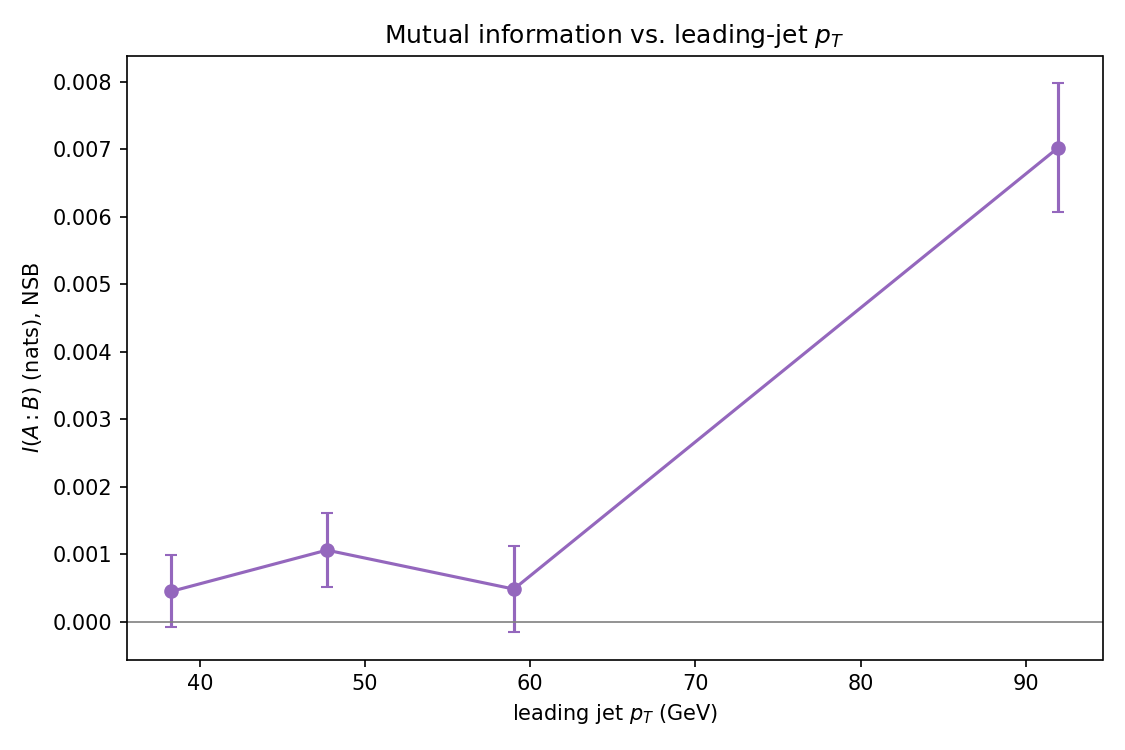
\includegraphics[width=0.8\textwidth]{figs/dijet_entropy_result_truth_MI_vs_pt.png}
\caption{PYTHIA~8: $I(A{:}B)$ (NSB) vs.\ leading-jet $p_T$.}
\label{fig:py-mi-pt}
\end{figure}

\begin{figure}[htb]
\centering
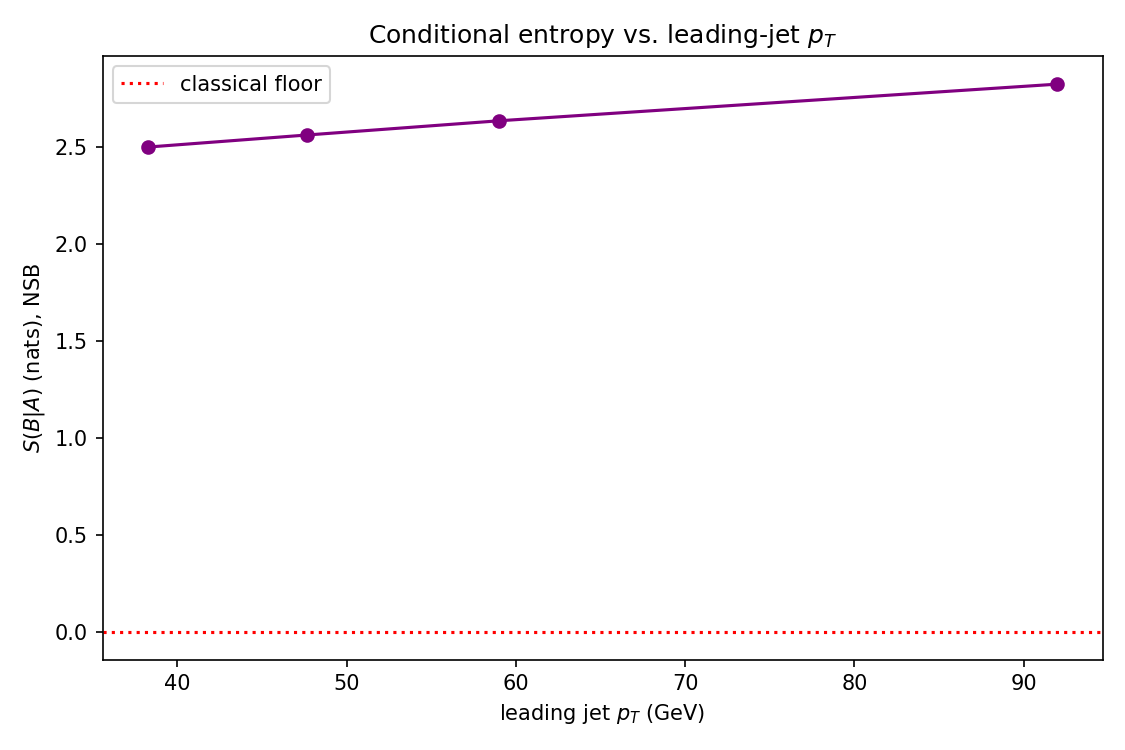
\includegraphics[width=0.8\textwidth]{figs/dijet_entropy_result_truth_SBA_vs_pt.png}
\caption{PYTHIA~8: $\SBA$ (NSB) vs.\ leading-jet $p_T$.}
\label{fig:py-sba-pt}
\end{figure}

\subsection{Multi-method comparison vs.\ $p_T$}

Figure~\ref{fig:py-method-comparison} overlays naive/Miller--Madow/
shuffle/NSB for $I(A{:}B)$, and naive/Miller--Madow/NSB for $\SBA$ (no
shuffle analogue, Sec.~\ref{sec:nsb}), each with bootstrap error bars
computed by the same unified procedure (Sec.~\ref{sec:sensitivity}). The
bias hierarchy naive~$>$~Miller--Madow~$\gtrsim$~NSB~$\approx$~shuffle
seen on the full sample (Fig.~\ref{fig:py-summary}) persists across
$p_T$ bins, most visibly in the highest-$p_T$ (lowest-statistics) bin,
where naive's upward bias is largest -- exactly the pattern the toy study
predicts for a bin with fewer events and a wider effective alphabet.

\begin{figure}[htb]
\centering
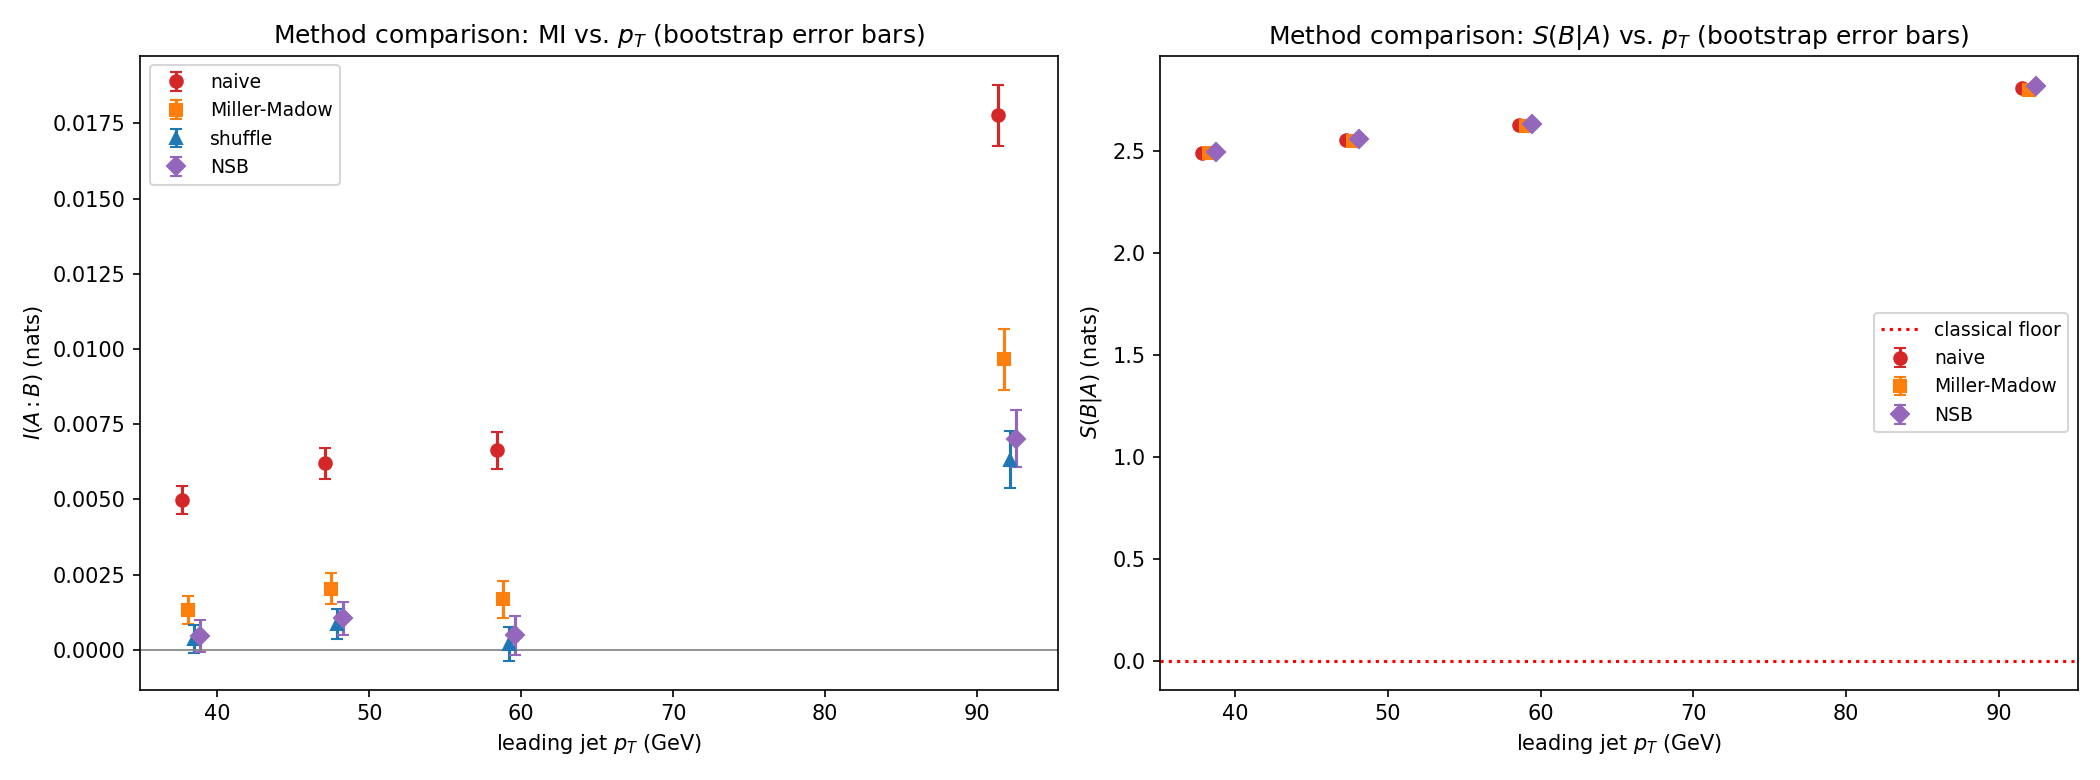
\includegraphics[width=\textwidth]{figs/dijet_entropy_result_truth_method_comparison_vs_pt.png}
\caption{PYTHIA~8: method comparison for $I(A{:}B)$ (left) and $\SBA$
(right) vs.\ leading-jet $p_T$, bootstrap error bars throughout.}
\label{fig:py-method-comparison}
\end{figure}

\subsection{Cross-validation with an independent implementation, and
normalized mutual information}
\label{sec:pythia-nmi}

The full pipeline was independently re-implemented in ROOT/C++ (own
validated digamma/trigamma special functions, own NSB posterior
computation, own bootstrap machinery) as a cross-check against the
Python implementation above, applied to the \emph{same} generated event
sample ($N\approx1.9\times10^5$, identical to
Secs.~\ref{sec:pythia}--\ref{sec:pythia-ptdep}). This section reports the
ROOT pipeline's results for $\NMI$ (Sec.~\ref{sec:observable}), which
were not part of the original Python-only analysis above.

Figure~\ref{fig:py-nmi-pt} shows $\NMI$ (NSB) vs.\ leading-jet $p_T$: all
values sit at $\NMI\ll1$, far below the classical bound, consistent with
the small $I(A{:}B)$ values already seen in absolute terms
(Fig.~\ref{fig:py-mi-pt}) and, as before, expected and unsurprising for a
classical event generator. The value of $\NMI$ here is methodological
rather than a physics result on this dataset: it demonstrates the
normalized witness is measurable with the same NSB machinery as $I$ and
$\SBA$, and (Sec.~\ref{sec:pitfall} below) that doing so correctly
requires some care.

\begin{figure}[htb]
\centering
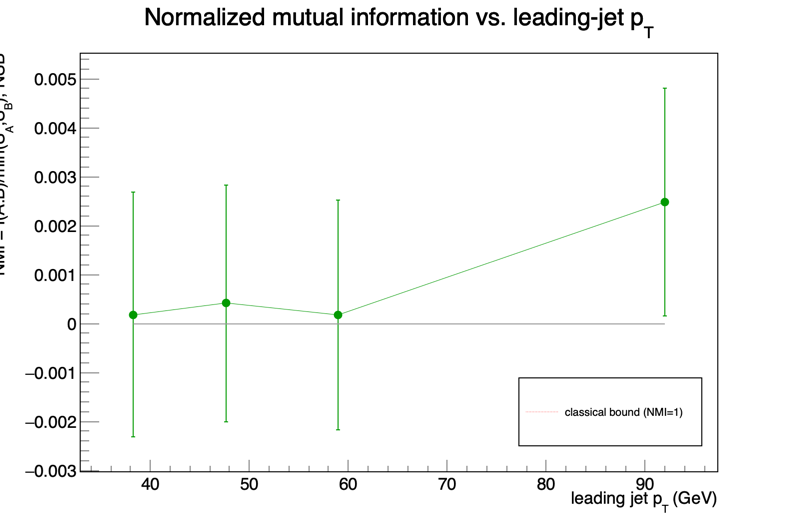
\includegraphics[width=0.8\textwidth]{figs/root_NMI_vs_pt.png}
\caption{PYTHIA~8 (ROOT implementation): $\NMI=I(A{:}B)/\min(S_A,S_B)$
(NSB) vs.\ leading-jet $p_T$. All values are far below the classical
bound $\NMI=1$, as expected for a classical event generator.}
\label{fig:py-nmi-pt}
\end{figure}

\subsection{A methodological pitfall: consistent uncertainty propagation
for derived ratios}
\label{sec:pitfall}

During development, the ROOT pipeline's multi-method comparison plot for
$\NMI$ (the $\NMI$ analogue of Fig.~\ref{fig:py-method-comparison}) showed
NSB error bars roughly $5$--$6\times$ larger, relative to the central
value, than NSB's own error bars on $I(A{:}B)$ in the immediately
adjacent panel (Fig.~\ref{fig:root-nmi-bug}, left) -- despite both
quantities being built from the same $S_A,S_B,S_{AB}$ on the same events.
Tracing this down surfaced a genuine implementation bug, worth recording
here since it is a general pitfall for any bootstrap-based uncertainty on
a \emph{derived, nonlinear} quantity (a ratio, in this case), not
specific to this codebase.

\paragraph{The bug.} $I(A{:}B)$'s bootstrap uncertainty was correctly
computed by resampling the event sample $N_{\rm boot}$ times and
recomputing $I$ fresh on each resample. $\NMI$'s point estimate used the
same procedure, but its \emph{uncertainty} was accidentally taken from an
older, separate analytic error-propagation formula (independence
approximation on $\mathrm{Var}(I)$ and $\mathrm{Var}(\min(S_A,S_B))$
combined in quadrature) left over from an earlier version of the
pipeline -- a different, more conservative methodology than the bootstrap
used for $I$ and $\SBA$ in the very same function, silently mixed into
one comparison plot.

\paragraph{The fix.} $\NMI$ is now bootstrapped exactly like $I$ and
$\SBA$: each resample's already-computed $S_A,S_B$ (needed anyway for
that resample's $I$) are reused to form $\NMI_{\rm resample} =
I_{\rm resample}/\min(S_{A,\rm resample},S_{B,\rm resample})$, and the
spread of $\NMI_{\rm resample}$ across resamples gives its uncertainty --
at no extra computational cost, since $S_A,S_B$ were already being
computed for $I$'s own bootstrap. Figure~\ref{fig:root-nmi-bug} illustrates
the discrepancy that led to identifying this;
Figure~\ref{fig:root-nmi-fixed} confirms the fix.

\begin{figure}[htb]
\centering
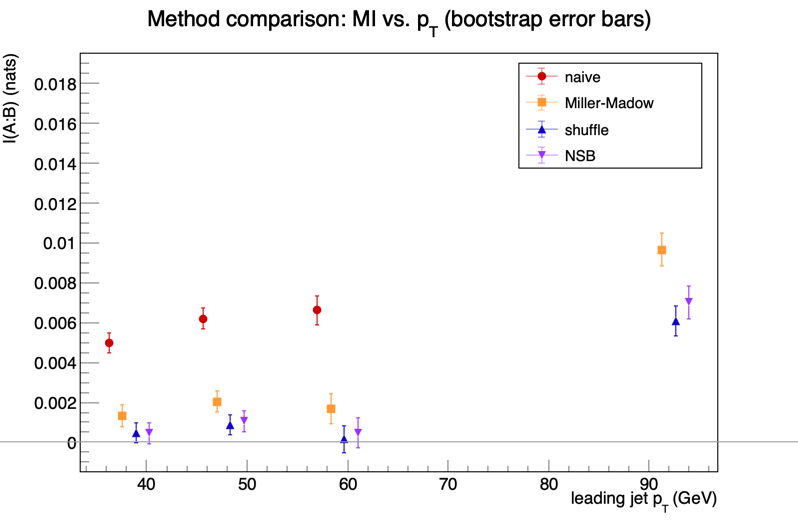
\includegraphics[width=0.48\textwidth]{figs/root_method_comparison_MI_vs_pt.png}
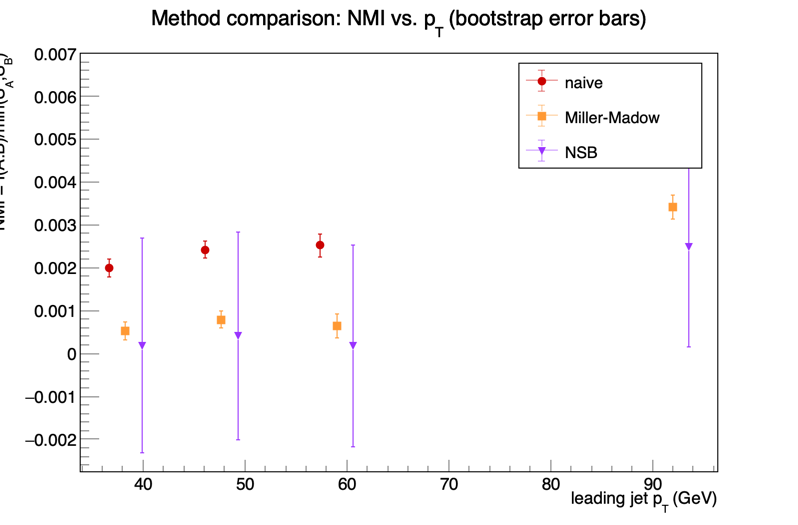
\includegraphics[width=0.48\textwidth]{figs/root_method_comparison_NMI_vs_pt_BUGGY.png}
\caption{The bug, illustrated: $I(A{:}B)$ method comparison (left,
unaffected) alongside the \emph{pre-fix} $\NMI$ method comparison (right)
from the same pipeline run. NSB's $\NMI$ error bars are visibly far wider,
relative to the central values, than $I$'s -- despite both being derived
from the same underlying quantities on the same events. This
discrepancy was the symptom that led to identifying the mixed-methodology
bug described in the text.}
\label{fig:root-nmi-bug}
\end{figure}

\begin{figure}[htb]
\centering
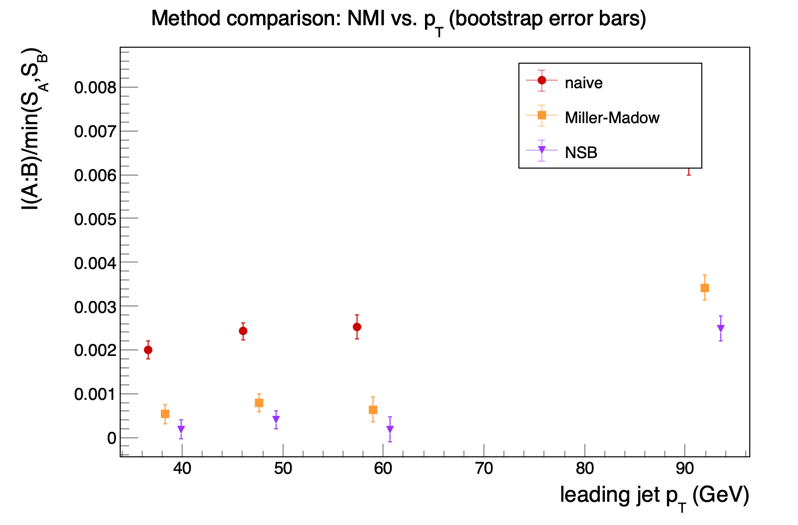
\includegraphics[width=0.48\textwidth]{figs/root_method_comparison_NMI_vs_pt_FIXED.png}
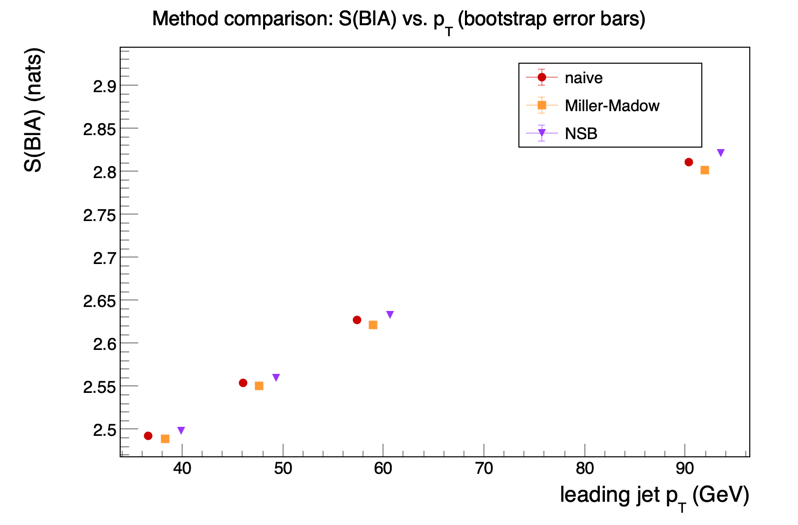
\includegraphics[width=0.48\textwidth]{figs/root_method_comparison_SBA_vs_pt.png}
\caption{Post-fix confirmation, same pipeline and dataset as
Fig.~\ref{fig:root-nmi-bug}: $\NMI$ method comparison (left) now shows
NSB error bars comparable in relative size to naive/Miller--Madow's, in
line with $I(A{:}B)$'s panel in Fig.~\ref{fig:root-nmi-bug} -- the
mixed-methodology discrepancy is gone. $\SBA$ method comparison (right,
never affected by this particular bug) shown alongside for reference,
confirming consistent bootstrap behavior across all three quantities.}
\label{fig:root-nmi-fixed}
\end{figure}

\paragraph{The general lesson.} When an uncertainty is obtained by
bootstrap resampling, every derived quantity built from the same
underlying estimate should be bootstrapped \emph{together, from the same
resamples} -- not by mixing bootstrap for some derived quantities and
analytic error propagation for others, even when both individually seem
reasonable. This also happens to be the more \emph{correct} choice
statistically, not merely the more consistent one: bootstrapping a ratio
directly captures the true correlation between numerator and denominator
(both estimated from the same event sample), whereas independence-
approximation error propagation assumes that correlation away and is
therefore both methodologically inconsistent \emph{and} typically
biased toward overly conservative (too large) uncertainties. This
pitfall generalizes beyond $\NMI$: any pipeline computing multiple
derived statistics from one bootstrap procedure should verify that
\emph{all} of them are actually using the same resamples, not just that
each individually looks plausible.

% =============================================================================
\section{Tier-2 closure test: calibrating estimator uncertainty on
realistic data}
\label{sec:closure}
% =============================================================================

The toy study (Secs.~\ref{sec:toymc}--\ref{sec:sensitivity}) validates
the estimator suite against a \emph{known} true MI, by construction. Real
PYTHIA~8 output, and eventually real STAR/ALICE data, has no such known
truth to validate against directly. This section describes a closure test
that closes that gap as far as is practically possible: calibrate a
synthetic model \emph{to resemble the real data}, use that model to
generate a pseudo-truth precise enough to treat as exact, and check
whether the estimator pipeline recovers it under closure -- i.e.\ under
exactly the statistical conditions (sample size, alphabet, correlation
strength) of the real measurement.

\subsection{Method}
\label{sec:closure-method}

\begin{enumerate}
\item \textbf{Calibrate.} Fit the toy study's Gamma-Poisson shared-latent
model (Sec.~\ref{sec:toymc}: $\Lambda\sim\mathrm{Gamma}(k,\theta)$,
$N_A|\Lambda\sim\mathrm{Poisson}(\Lambda)$,
$N_B|\Lambda\sim\mathrm{Poisson}(c\Lambda)$) to the \emph{real} data's
five leading moments -- $\langle N_A\rangle,\mathrm{Var}(N_A),
\langle N_B\rangle,\mathrm{Var}(N_B),\mathrm{Corr}(N_A,N_B)$ -- via
least squares over $(k,\theta,c)$. This is a genuine, honest constraint:
a 3-parameter model cannot exactly match 5 targets in general, and the
achieved fit quality is reported explicitly rather than assumed.
\item \textbf{Establish a pseudo-truth.} Draw a very large sample
(typically $10^6$--$5\times10^6$ events) from the \emph{fitted} model.
At this scale the naive estimator's own bias
($\mathcal{O}(1/N)$, Sec.~\ref{sec:bias}) is negligible, so $I,\SBA,\NMI$
computed on this sample are treated as numerically exact
($I_{\rm true},\SBA_{\rm true},\NMI_{\rm true}$) -- calibrated to
resemble the real measurement's shape and correlation strength, not an
arbitrary toy scenario.
\item \textbf{Closure.} Draw $N_{\rm repeats}$ independent fresh samples
from the fitted model, each at the real dataset's actual event count $N$
(and using the real analysis's alphabet), and run the full
naive/Miller--Madow/shuffle/NSB pipeline on each.
\item \textbf{Check bias and calibration.} For NSB specifically, form the
\emph{pull} for each repeat,
$z = (\hat X_{\rm NSB}-X_{\rm true})/\sigma_{\rm NSB}$
for $X\in\{I,\SBA,\NMI\}$, using that repeat's own bootstrap
$\sigma_{\rm NSB}$ (Sec.~\ref{sec:pitfall}). If the estimator is unbiased
and its uncertainty well-calibrated, the pull distribution across repeats
should be standard normal: mean $0$, standard deviation $1$, with
$\sim\!68\%$ of repeats within $\pm1\sigma$ and $\sim\!95\%$ within
$\pm2\sigma$.
\end{enumerate}
This is purely diagnostic throughout -- no bias or coverage correction is
applied to any reported number anywhere in this note; the closure test's
role is to establish \emph{whether} the raw bootstrap uncertainty can be
trusted at face value for a given $(N,\text{alphabet})$, not to patch it.

\subsection{Whole-sample results}
\label{sec:closure-results}

Applying this to the full $14$~TeV validation sample
(Fig.~\ref{fig:closure-I}, $I(A{:}B)$; Fig.~\ref{fig:closure-nmi}, $\NMI$)
gives two consistent findings:

\begin{itemize}
\item \textbf{A mean pull of approximately $-1$}: NSB systematically
under-\emph{estimates} $I(A{:}B)$ (and correspondingly $\NMI$) by
roughly one of its own reported bootstrap-$\sigma$'s, on average, at this
sample's statistics. This is a real, non-negligible bias, though modest
in scale.
\item \textbf{A pull standard deviation of approximately $1.5$--$1.7$}:
the \emph{actual} spread of $(\hat X-X_{\rm true})$ across independent
repeats is $50$--$70\%$ \emph{larger} than what the reported bootstrap
$\sigma$ claims. In other words, \texttt{NSB} $\pm$ \texttt{bootstrap
$\sigma$} under-covers -- the quoted error bars are too tight. A
significance computed naively from the raw bootstrap $\sigma$ at this
$(N,\text{alphabet})$ therefore overstates the true significance by
roughly this same factor (e.g.\ a naive $3\sigma$ claim would correspond
to a true significance closer to $3/1.7\approx1.8\sigma$).
\end{itemize}
The pull distributions in both figures are also visibly non-Gaussian:
skewed, with a heavier negative tail extending to several $\sigma$ beyond
what a standard normal would predict, rather than a uniformly-widened but
still-symmetric Gaussian. This matters practically: a single multiplicative
correction to $\sigma$ (calibrating only the second moment) would not
fully correct the shape of the tail, which is the part most relevant to a
discovery-level claim specifically. Any downstream use of these
bootstrap uncertainties for a significance statement should treat this as
a known, quantified limitation rather than an assumption to be taken on
faith -- exactly the purpose of running this closure test before, not
after, a real measurement.

\begin{figure}[htb]
\centering
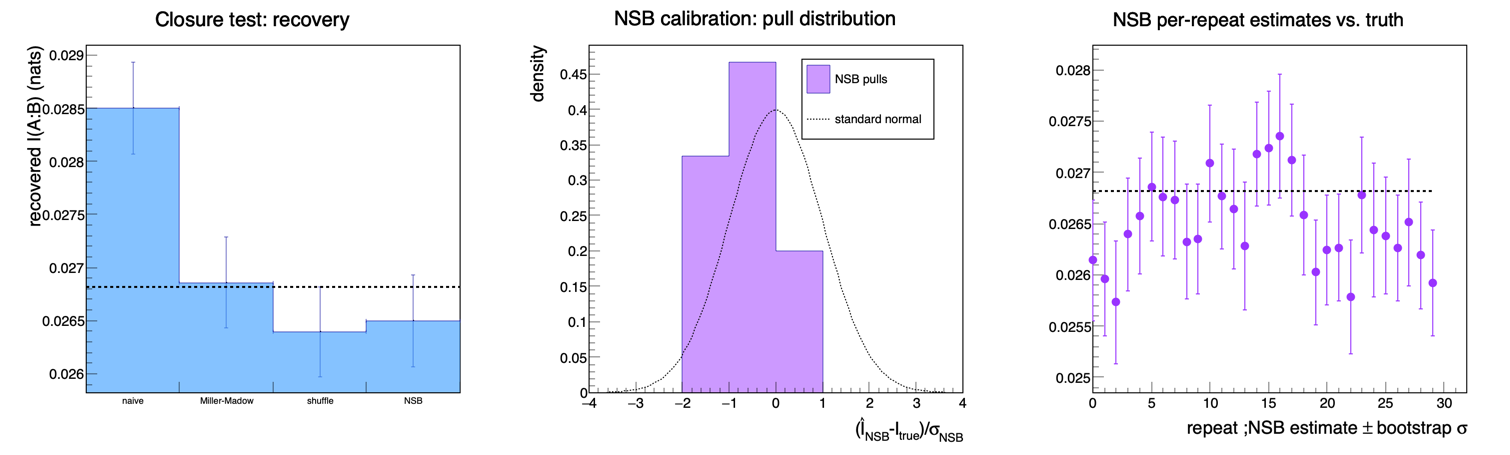
\includegraphics[width=\textwidth]{figs/closure_test_I.png}
\caption{Whole-sample closure test, $I(A{:}B)$: recovery across methods
(left), NSB pull distribution vs.\ standard normal (center), per-repeat
NSB estimates vs.\ the fitted-model pseudo-truth (right).}
\label{fig:closure-I}
\end{figure}

\begin{figure}[htb]
\centering
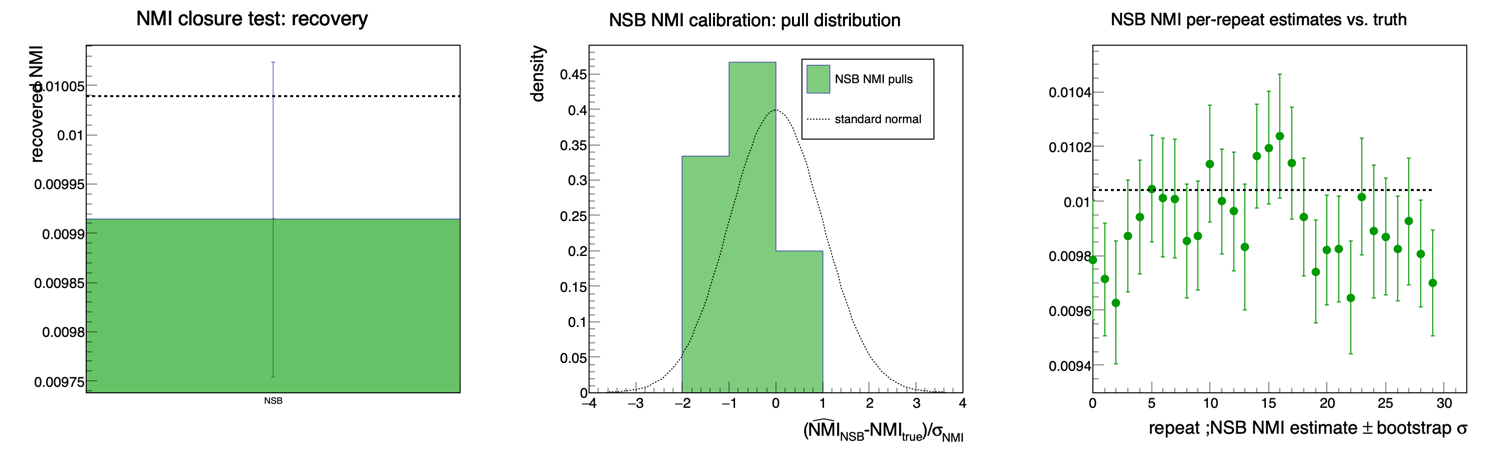
\includegraphics[width=\textwidth]{figs/closure_test_NMI.png}
\caption{Whole-sample closure test, $\NMI$: same three panels as
Fig.~\ref{fig:closure-I}, for the normalized witness.}
\label{fig:closure-nmi}
\end{figure}

\subsection{Extension to the conditional-entropy witness directly}
\label{sec:closure-sba}

Sections~\ref{sec:closure-method}--\ref{sec:closure-results} were run
for $I(A{:}B)$ and $\NMI$; since $\SBA$ is the quantity that would
actually carry a quantum-witness claim, a dedicated closure test for
$\SBA$ itself (mean pull, pull standard deviation, and calibration
fraction within $\pm1\sigma/\pm2\sigma$, identical procedure to
Sec.~\ref{sec:closure-method}) has been implemented and is not inferred
from $I$'s behavior via $\SBA=S_B-I(A{:}B)$ -- that inference would
carry $S_B$'s own separate estimation noise and is not a substitute for
a direct check.

Figure~\ref{fig:closure-sba} shows the result on the same $14$~TeV
validation sample. Qualitatively it differs from $I$/$\NMI$
(Sec.~\ref{sec:closure-results}) in both sign and tightness: the pull
distribution is concentrated at small \emph{positive} values (peak in
the $[0,1]$ bin, most mass within $[-1,2]$) rather than the leftward
skew seen for $I$/$\NMI$, indicating a modest positive bias -- NSB
tends to slightly \emph{over}-estimate $\SBA$ here, the opposite
direction from $I$'s under-estimate -- and the spread is visibly
tighter, closer to a well-calibrated pull std of order $1$ than the
$1.5$--$1.7$ found for $I$/$\NMI$. This is a genuinely different
calibration behavior for the two quantities on the same sample, not a
restatement of the same number, and is exactly why this check could not
be skipped in favor of inferring $\SBA$'s calibration from $I$'s.

\begin{figure}[htb]
\centering
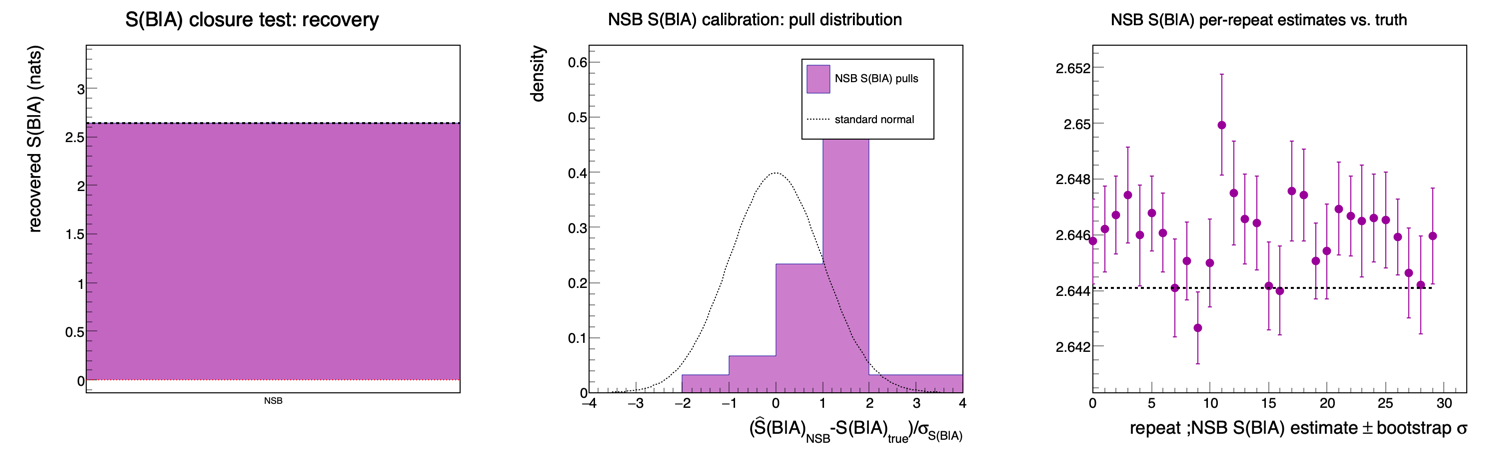
\includegraphics[width=\textwidth]{figs/closure_test_SBA.png}
\caption{Whole-sample closure test, $\SBA$: same three panels as
Fig.~\ref{fig:closure-I}, for the conditional-entropy witness. Note the
positive pull skew and tighter spread compared to $I$/$\NMI$
(Fig.~\ref{fig:closure-I}--\ref{fig:closure-nmi}).}
\label{fig:closure-sba}
\end{figure}

\subsection{$p_T$-differential closure test}
\label{sec:closure-pt}

The results of Sec.~\ref{sec:closure-results} calibrate NSB's uncertainty
for a dataset shaped like the \emph{whole} sample -- but both the
underlying multiplicity/correlation structure and the per-bin event count
change with $p_T$ (Secs.~\ref{sec:pythia-ptdep},
\ref{sec:pythia}--\ref{sec:pythia-nmi}), so whole-sample calibration does
not automatically transfer to any individual $p_T$ bin, particularly the
highest-$p_T$, lowest-statistics bins where a genuine signal would be
most interesting and least well-measured. A $p_T$-differential extension
of the closure test has been implemented: for each $p_T$ bin
independently, fit a bin-specific Gamma-Poisson model to that bin's own
events (not the whole-sample fit), generate a bin-specific pseudo-truth,
and run the closure procedure at that bin's actual event count --
directly answering ``is NSB's uncertainty trustworthy in \emph{this}
bin'' rather than assuming the whole-sample answer applies uniformly.

Figure~\ref{fig:closure-pt-summary} shows the result, in the same four
$p_T$ bins used throughout Sec.~\ref{sec:pythia-ptdep} ($p_T$ centers
$\approx38,48,59,92$~GeV). The pattern is notably different from, and in
one respect more encouraging than, the whole-sample result of
Sec.~\ref{sec:closure-results}:

\begin{itemize}
\item \textbf{Pull means} for $I(A{:}B)$ and $\NMI$ are small and
negative throughout ($\approx-0.12$ to $-0.17$ in the three lower-$p_T$
bins, shrinking to $\approx-0.04$ in the highest-$p_T$ bin) -- markedly
smaller in magnitude than the whole-sample $\approx-1$ found in
Sec.~\ref{sec:closure-results}. $\SBA$'s pull mean is somewhat larger at
low $p_T$ ($\approx-0.29$) but trends toward zero as $p_T$ increases,
reaching $\approx0$ in the highest-$p_T$ bin.
\item \textbf{Pull standard deviations} for $I(A{:}B)$ and $\NMI$ rise
from $\approx0.58$ (lowest-$p_T$ bin, i.e.\ \emph{over}-covering -- the
bootstrap $\sigma$ is if anything too conservative there) through
$\approx0.80$ and $\approx0.95$ to $\approx0.92$ in the highest-$p_T$
bin -- staying at or below $1$ throughout, in contrast to the
whole-sample $1.5$--$1.7$ under-covering. $\SBA$'s pull standard
deviation is close to $1$ in every bin ($\approx1.02,1.00,1.11,0.92$) --
the best-calibrated of the three quantities here, and encouragingly close
to ideal given $\SBA$ is the quantity that would carry an actual
discovery claim.
\end{itemize}

\begin{figure}[htb]
\centering
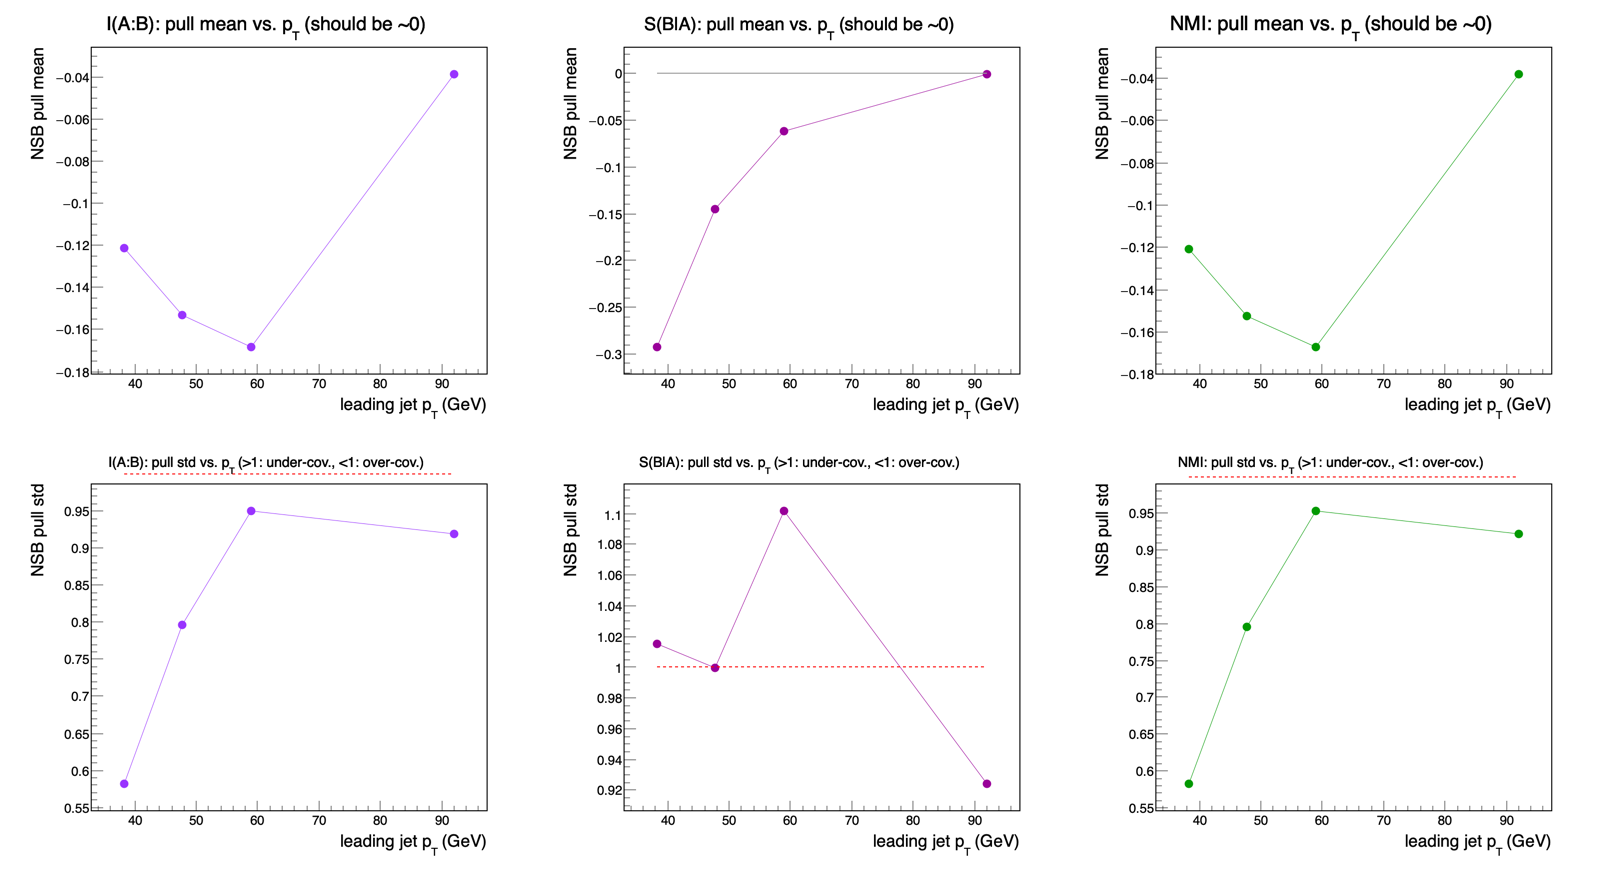
\includegraphics[width=\textwidth]{figs/closure_test_pt_summary.png}
\caption{$p_T$-differential closure test: NSB pull mean (top row) and
standard deviation (bottom row) vs.\ leading-jet $p_T$, for $I(A{:}B)$
(left), $\SBA$ (center), and $\NMI$ (right). Red dashed line marks
perfect calibration (pull std $=1$).}
\label{fig:closure-pt-summary}
\end{figure}

This bin-by-bin result being better-calibrated than the whole-sample one
is itself a meaningful, self-consistent finding, not merely a nicer
number: Sec.~\ref{sec:closure-pt}'s entire motivation was that the
whole-sample Gamma-Poisson fit has to compromise across a range of
$p_T$-dependent correlation structures at once (Sec.~\ref{sec:pythia-ptdep}),
whereas each bin-specific fit only has to describe its own,
comparatively homogeneous sub-population. A better-calibrated per-bin
result is exactly what that design difference predicts, and is evidence
the whole-sample closure test's miscalibration (Sec.~\ref{sec:closure-results})
is at least partly a model-fit-quality effect specific to forcing one
3-parameter model to span the full $p_T$ range, rather than a property of
NSB's bootstrap uncertainty in general. That said, this is a single
validation dataset at one set of statistics; whether this pattern holds
at STAR's actual $200$~GeV kinematics and statistics
(Sec.~\ref{sec:conclusions}) is not yet established and should not be
assumed.

Even with this more encouraging per-bin picture, no bin here reaches
pull std $=1$ exactly, and the lowest-$p_T$ bin's over-covering for
$I$/$\NMI$ ($\approx0.58$) is itself a $\sim\!40\%$ deviation from ideal
calibration, in the conservative direction. The practical recommendation
of Sec.~\ref{sec:closure-results} therefore still stands as the safe
default -- treat raw bootstrap $\sigma$ with caution and consult a
closure test at the actual bin/statistics in use -- with this section's
result showing that the correction, at least for this validation sample,
tends to be smaller and bidirectional per bin rather than a uniform
large under-coverage.

% =============================================================================
\section{A distinct systematic: trivial kinematic MI, and its removal by
mixed-event subtraction}
\label{sec:mixed}
% =============================================================================

Everything so far corrects \emph{estimator} bias: the gap between a
finite-sample MI estimate and the true MI of the sample's generating
distribution. This section addresses a different problem, upstream of
estimation entirely -- a sense in which the \emph{true} MI being
estimated is itself partly an artifact of the measurement's finite
$p_T$ binning, not a real dynamical correlation.

\subsection{The problem}

Both jets' multiplicities depend on their own $p_T$
(Sec.~\ref{sec:pythia-ptdep}), and $p_{T,1}$, $p_{T,2}$ are themselves
correlated through momentum balance. This is a common-cause structure:
even if $N_A$ and $N_B$ were completely independent \emph{conditional
on} the event kinematics, integrating over any $p_T$ window of finite
width induces real, nonzero $I(A{:}B)$ -- not estimator bias, genuine
correlation, but kinematically trivial and present in a purely classical
generator with no dynamical jet--jet correlation at all. This does not
vanish for any finite bin width, only shrinks as the bin narrows; the
quantity one actually wants is closer to the conditional mutual
information $I(N_A{:}N_B \mid p_T)$, which finite-width binning only
approximates from above. Notably, this problem does \emph{not} affect
the quantum-witness test itself ($\SBA<0$ or $\NMI>1$): trivial
kinematic correlation can only push a measurement deeper into the
classical region, never fake a violation. It matters specifically for
interpreting the \emph{magnitude} of a measured $I(A{:}B)$ as evidence
of dynamical (as opposed to purely kinematic) correlation.

\subsection{Mixed-event subtraction}

For each event, jet A's multiplicity and kinematics are kept as
measured; jet B's multiplicity is replaced with that of a
\emph{different} event's jet B, selected by $k$-nearest-neighbor
matching in $p_{T,2}$ (default $k=10$). Mixed pairs then reproduce the
same kinematic structure as the same-event sample, but with $N_B$ drawn
conditionally independent of $N_A$ given (matched) kinematics -- so the
mixed sample's own MI, $I_{\rm mix}$, directly estimates the trivial
kinematic contribution. The beyond-kinematics signal is
\begin{equation}
I_{\rm signal} \;=\; I^{\rm corrected}_{\rm same} - I^{\rm corrected}_{\rm mix}\,,
\end{equation}
with bias correction applied to \emph{each term separately} -- not to
the already-subtracted difference, which would double-correct, since
the leading naive bias $\approx(K_{AB}-K_A-K_B+1)/(2N)$ largely cancels
between the two terms already (same marginals and same $N$ by
construction). Uncertainties are obtained by a \emph{joint} bootstrap of
the full difference: each resample rebuilds both the same-event pairs
and the mixed pairs (re-matching within the resample) and recomputes
$I_{\rm same}-I_{\rm mix}$ for all four methods, never propagating the
two terms' errors separately -- the same lesson as
Sec.~\ref{sec:pitfall}, and more important here since the two terms
share events and are strongly correlated. The matching resolution $k$ is
itself a systematic: any residual within-window $p_T$ variation remains
unsubtracted trivial MI, and varying $k$ and checking stability of
$I_{\rm signal}$ is the natural check.

\subsection{Relation to shuffle-subtraction}

The two corrections are not redundant, though they are the same
operation at different resolutions. Shuffling permutes $N_B$ labels
\emph{within the analysis sample}, which realizes the product of that
sample's own marginals -- exactly what mixed-event pairing gives in the
limit of no kinematic matching at all ($k\to$ the full sample).
Formally: \emph{shuffle-subtraction is mixed-event subtraction with
matching resolution equal to the analysis bin}. What differs is the
null each realizes, and so what each subtraction removes: shuffling's
null has true MI exactly zero, so it corrects only finite-sample
estimator bias and deliberately leaves all real correlation --
including the trivial kinematic part -- intact. Fine-matched mixing's
null has nonzero true MI (the trivial kinematic part), so it removes a
genuine physical contribution. The two are complementary, not
alternatives: bias correction (via shuffle, Miller--Madow, or NSB) is
applied to each of $I_{\rm same}$ and $I_{\rm mix}$ individually, and
the kinematic subtraction is taken between the two corrected numbers.

\subsection{Validation: bias near-cancellation and closure test}

Figure~\ref{fig:mixed-qa} first validates the construction on a
purpose-built synthetic dataset with $N_A\perp N_B \mid p_T$ exactly by
construction (a shared momentum-balance kinematic correlation with no
dynamical jet--jet correlation added) -- a case where $I_{\rm signal}$
should recover zero. The raw same-event MI is entirely trivial
($\approx0.034$--$0.039$ nats depending on method) yet the mixed-event
difference is consistent with zero for every one of naive,
Miller--Madow, shuffle, and NSB. The near-cancellation predicted above
is directly visible: the \emph{raw} naive same-event and mixed-event
estimates individually carry substantial bias ($0.0386$ vs.\ a true
value near zero), but naive-minus-naive
($-0.00132$) lands almost on top of NSB-minus-NSB ($-0.00140$) --
the bias has canceled between the two terms to within the bootstrap
uncertainty, before any explicit correction was applied at all.

\begin{figure}[htb]
\centering
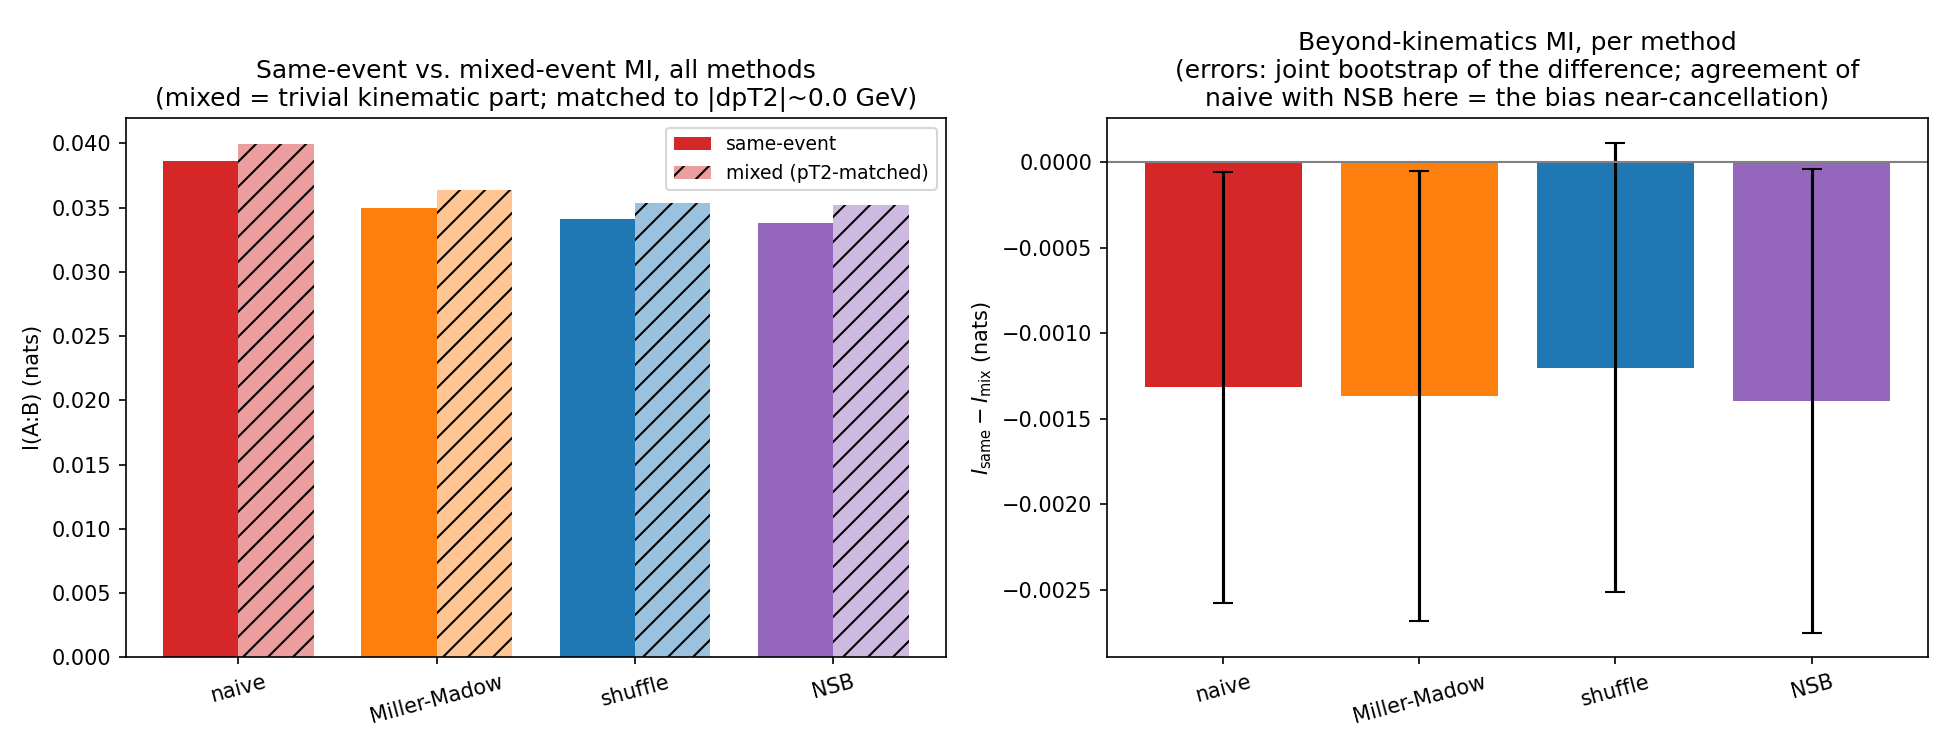
\includegraphics[width=\textwidth]{figs/mixed_qa_synthetic.png}
\caption{Mixed-event subtraction QA on a synthetic dataset with
$N_A\perp N_B\mid p_T$ by construction. Left: same-event vs.\
$p_{T,2}$-matched mixed-event $I(A{:}B)$, all four methods -- both are
dominated by the trivial kinematic contribution. Right: the per-method
difference with jointly-bootstrapped errors, consistent with zero
throughout; naive-minus-naive agreeing with NSB-minus-NSB despite the
raw naive terms' visible individual bias is the near-cancellation
described in the text.}
\label{fig:mixed-qa}
\end{figure}

This motivated a dedicated closure test for the subtraction itself,
distinct from Sec.~\ref{sec:closure}'s closure tests for the raw
estimators. The model resamples $(p_{T,1},p_{T,2})$ pairs directly from
real data (reproducing the true kinematic correlation exactly, no
spectrum model needed), fits $\lambda_j(p_T)=a_j+b_j\ln p_T$ to each
jet's real multiplicity--$p_T$ profile, and injects a controllable
\emph{genuine} beyond-kinematics correlation via a shared latent
$g\sim\mathrm{Gamma}(1/s^2,s^2)$ multiplying both jets' rates ($s=0$:
exactly conditionally independent, true signal exactly zero; $s>0$: a
known injected signal). Pseudo-truth is obtained from a large reference
sample analyzed with the identical matched-mixing procedure, so the
truth is defined for exactly the estimand the method targets.

Unlike the reduced-statistics smoke test reported in an earlier
revision of this note, Figs.~\ref{fig:closure-mixed-null-real}--\ref{fig:closure-mixed-signal-real}
show the closure test run at full statistics ($30$ repeats, $30$-fold
joint bootstrap per repeat) directly on the real $14$~TeV validation
sample's own fitted kinematics and multiplicity profile -- both
scenarios required by the design (Sec.~\ref{sec:mixed}): the
\emph{null} ($s=0$), the essential false-positive control before
claiming any beyond-kinematics signal on real data, and an
injected-signal case ($s=0.15$).

\begin{figure}[htb]
\centering
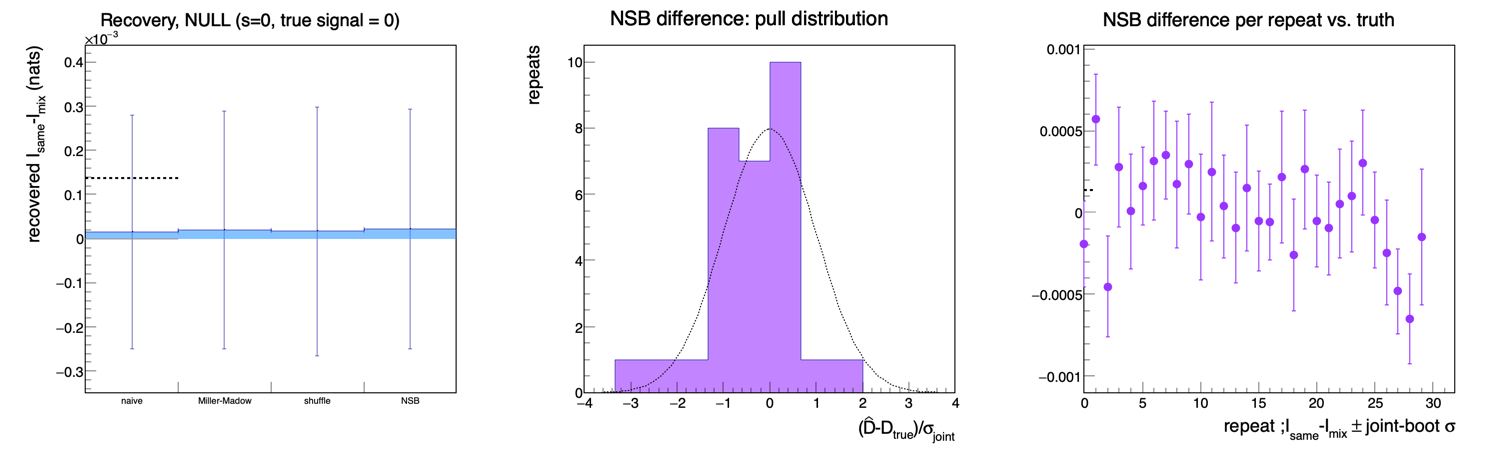
\includegraphics[width=\textwidth]{figs/closure_mixed_null_real.png}
\caption{Closure test of the mixed-event subtraction on the real $14$~TeV
validation sample's fitted kinematics, null scenario ($s=0$), full
statistics ($30$ repeats). Left: recovered $I_{\rm same}-I_{\rm mix}$ per
method vs.\ the (near-zero) pseudo-truth. Center: NSB-difference pull
distribution against standard normal. Right: per-repeat NSB estimates
with joint-bootstrap error bars vs.\ the true value.}
\label{fig:closure-mixed-null-real}
\end{figure}

\begin{figure}[htb]
\centering
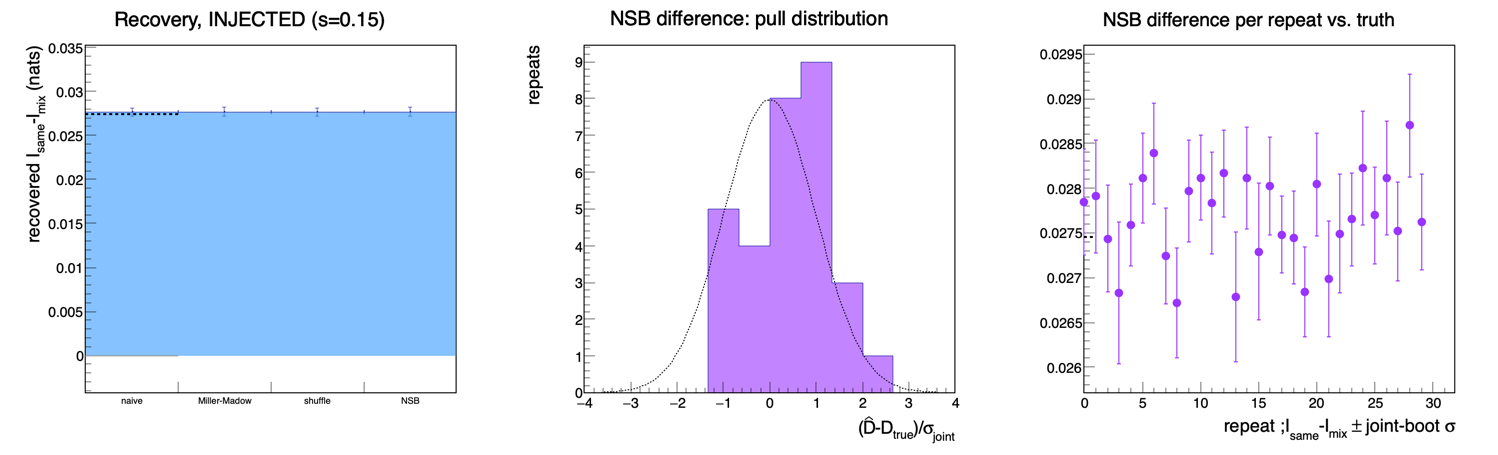
\includegraphics[width=\textwidth]{figs/closure_mixed_signal_real.png}
\caption{Same as Fig.~\ref{fig:closure-mixed-null-real}, injected-signal
scenario ($s=0.15$, true difference $\approx0.0275$ nats).}
\label{fig:closure-mixed-signal-real}
\end{figure}

In the null scenario the pseudo-truth itself is small but not exactly
zero ($\approx1.4\times10^{-4}$ nats) -- expected, since it is estimated
by the naive estimator on a large but finite reference sample and
carries that estimator's own residual $\mathcal{O}(1/N)$ noise, not a
flaw in the null construction. All four methods recover values
consistent with this truth within their (comparatively large, since the
true difference is itself tiny) joint-bootstrap uncertainties, and the
NSB-difference pull distribution does not show the pronounced skew seen
in the raw-estimator whole-sample closure tests
(Sec.~\ref{sec:closure-results}). In the injected-signal scenario, all
four methods recover the true $\approx0.0275$~nats difference closely
and consistently, again without the earlier tests' marked
under-coverage. Taken together, the mixed-event \emph{difference}
appears better-calibrated at these statistics than the raw single-term
estimators were -- plausibly because the joint bootstrap directly
captures the strong correlation between the same-event and mixed-event
terms (they share events), which the raw single-quantity closure tests
had no analogue of. This is an encouraging empirical finding rather
than a proven general property, and should not be assumed to hold
automatically at STAR's real kinematics and statistics without
rerunning this same check there.

\subsection{Application to the real validation sample}
\label{sec:mixed-real}

With the method validated, it was applied to the actual $14$~TeV
PYTHIA~8 validation sample used throughout Sec.~\ref{sec:pythia} --
answering the question Sec.~\ref{sec:mixed}'s design was motivated by:
how much of the $I(A{:}B)$ measured elsewhere in this note is trivial
kinematic correlation, versus a beyond-kinematics component.

\begin{figure}[htb]
\centering
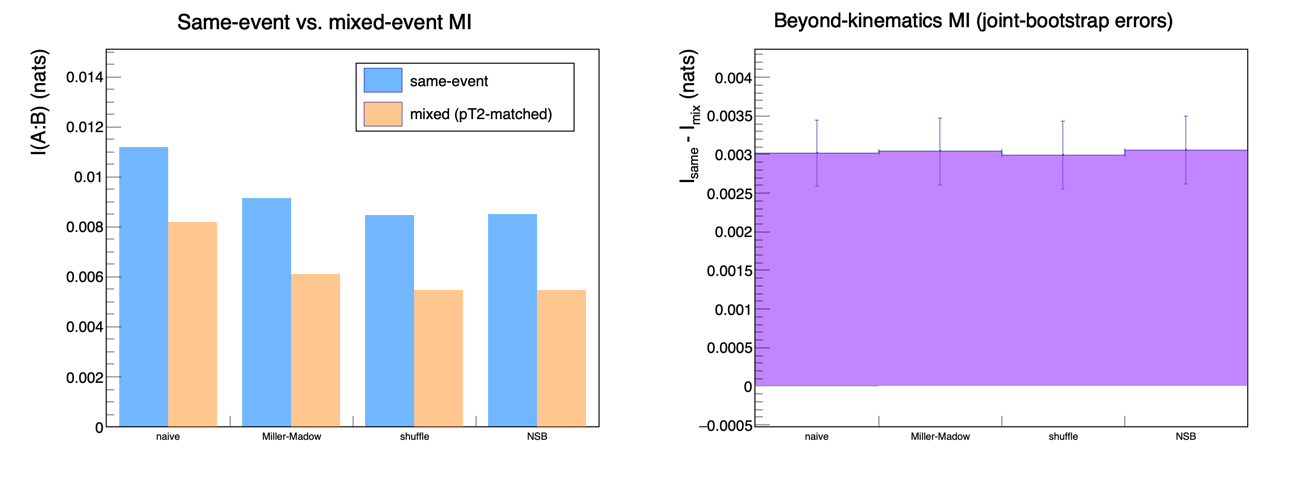
\includegraphics[width=\textwidth]{figs/mixed_qa_real.png}
\caption{Mixed-event subtraction applied to the real $14$~TeV validation
sample (whole sample). Left: same-event vs.\ $p_{T,2}$-matched
mixed-event $I(A{:}B)$, all four methods. Right: the per-method
difference with jointly-bootstrapped errors -- a nonzero
beyond-kinematics component, consistently recovered across all four
estimators.}
\label{fig:mixed-real-qa}
\end{figure}

Figure~\ref{fig:mixed-real-qa} shows the whole-sample result. Same-event
$I(A{:}B)\approx0.0084$--$0.0112$~nats depending on method (naive
highest, as expected from its known upward bias), dropping to
$\approx0.0055$--$0.0082$~nats for the $p_{T,2}$-matched mixed sample.
The difference is $\approx0.0030$~nats, and -- notably -- essentially
\emph{the same} value across all four methods, with joint-bootstrap
uncertainty $\approx\pm0.0004$--$0.0005$~nats. Roughly
$60$--$70\%$ of the raw same-event MI is removed as trivial kinematic
correlation (depending slightly on method); the remaining
$\approx0.003$~nats is a genuine, nonzero beyond-kinematics signal, not
an artifact of any one estimator's bias.

Since PYTHIA~8 has no mechanism for quantum entanglement between
separately hard-scattered jets, this remaining correlation must be
classical in origin. The most likely candidate, anticipated already in
Sec.~\ref{sec:mixed}'s design discussion, is shared underlying-event
activity -- multiple-parton interactions, beam-remnant particles, and
color reconnection all act coherently on \emph{both} jets within the
same event, and matching mixed partners only on jet-B's $p_T$ does
nothing to remove event-level (as opposed to jet-level) shared
structure. This is consistent with, not a contradiction of, the
subtraction's design: the method isolates correlation beyond simple
$p_T$-driven kinematics, and underlying-event effects are exactly the
kind of genuine (if unglamorous) dynamical correlation that description
was always going to include.

\begin{figure}[htb]
\centering
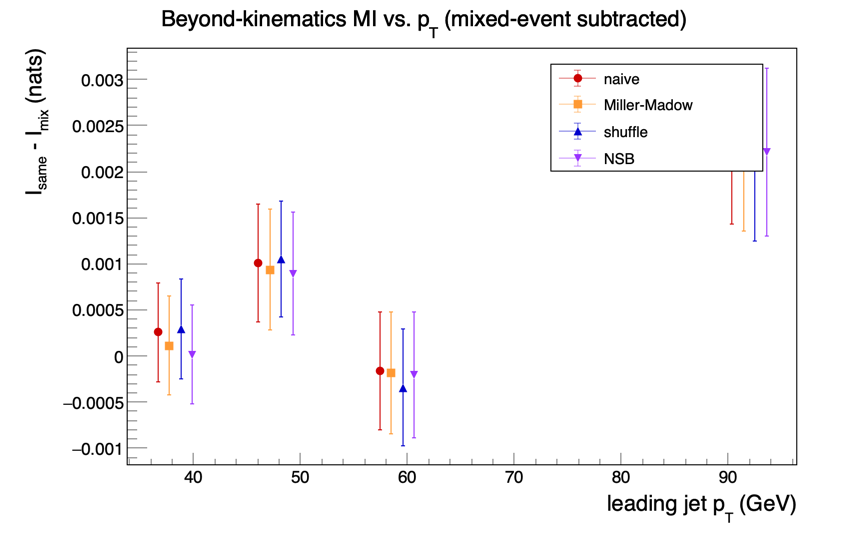
\includegraphics[width=0.75\textwidth]{figs/mixed_diff_vs_pt_real.png}
\caption{Beyond-kinematics MI vs.\ leading-jet $p_T$ (mixed-event
subtracted), real validation sample, all four methods.}
\label{fig:mixed-real-pt}
\end{figure}

The $p_T$-differential breakdown (Fig.~\ref{fig:mixed-real-pt}) is less
clean, as expected given each bin carries roughly a quarter of the
whole sample's statistics: the two lower-$p_T$ bins are consistent with
zero, the third bin shows a small positive value
($\approx0.0009$--$0.0011$~nats), and the highest-$p_T$ bin shows the
largest value ($\approx0.0015$--$0.0022$~nats) but also by far the
largest uncertainty. All four methods agree closely within each bin,
which is reassuring for the subtraction's internal consistency, but no
individual bin here should be read as an independently significant
detection -- the whole-sample result in Fig.~\ref{fig:mixed-real-qa},
with its higher statistics and tighter relative uncertainty, is the
more trustworthy number at this stage. A closure test run specifically
at each bin's statistics (the pT-differential analogue of
Sec.~\ref{sec:closure-pt}, not yet built for the mixed-event method)
would be needed before quoting a per-bin significance with confidence.

\subsection{Status and outlook}

The subtraction machinery, its bias-cancellation property, a
closure-test framework validating it at full statistics on the real
sample's own kinematics, and an application to the real validation
sample itself are now all complete
(Figs.~\ref{fig:mixed-qa}--\ref{fig:mixed-real-pt}). What remains: a
$p_T$-differential closure test for the mixed-event difference
specifically (paralleling Sec.~\ref{sec:closure-pt}'s extension of the
raw-estimator closure test), needed before the per-bin breakdown in
Fig.~\ref{fig:mixed-real-pt} can support a significance claim in any
individual bin; and, longer-term, isolating the underlying-event
contribution more directly (e.g.\ by matching on additional event
activity variables, not just jet-B's $p_T$) if a cleaner separation of
kinematic, underlying-event, and (eventually, on real detector data)
any genuinely anomalous component is wanted.


% =============================================================================
\section{Overall conclusions and next steps}
\label{sec:conclusions}
% =============================================================================

The toy Monte Carlo study (Secs.~\ref{sec:toymc}--\ref{sec:sensitivity})
establishes the estimator methodology and its failure modes under
controlled, known conditions. Section~\ref{sec:pythia} shows the same
pipeline, unmodified, correctly recovers physically-expected behavior
(NBD-like overdispersion, MLLA-consistent multiplicity growth with $p_T$,
the same finite-sample bias shape) on realistic QCD Monte-Carlo output
where no such structure was hand-built in -- a meaningful, if indirect,
validation that the pipeline is measuring real structure rather than an
artifact of the toy model's specific construction. An independent
ROOT/C++ re-implementation (Sec.~\ref{sec:pythia-nmi}) cross-validates the
Python results and adds $\NMI$, the scale-comparable normalized version
of the witness (Sec.~\ref{sec:observable}) needed to compare measurements
across $p_T$ bins, run periods, or collision energies on a common,
bounded scale.

That cross-validation also surfaced a genuine implementation bug
(Sec.~\ref{sec:pitfall}): a bootstrap-based derived quantity ($\NMI$)
picked up its uncertainty from an inconsistent, more conservative
analytic formula rather than the same resampling procedure used for
$I(A{:}B)$ and $\SBA$ in the same function. The fix, and more
importantly the general principle it illustrates -- every derived
quantity built from one bootstrap procedure must be resampled together,
not mixed with a separately-derived analytic error -- is recorded in
full since it is a pitfall relevant to any bootstrap-based entropy/MI
pipeline, not just this one.

Section~\ref{sec:closure} closes the gap the previous revision of this
note flagged as open: a closure test calibrated to resemble the real
PYTHIA~8 sample (Gamma-Poisson model fit to the real data's marginals and
correlation strength, huge reference sample for a pseudo-truth, repeated
closure at the real dataset's actual statistics) finds that NSB's
bootstrap uncertainty, at this sample's $(N,\text{alphabet})$, is
\textbf{under-covering by a factor of roughly $1.5$--$1.7$}, with a mean
bias of order $-1\sigma$ and a pull distribution that is skewed rather
than symmetrically widened. This is a quantitative, load-bearing result
for any future significance claim: a naive $3\sigma$ excess computed from
raw bootstrap $\sigma$ at comparable statistics should be read as
$\sim\!1.8$--$2\sigma$ once this calibration factor is accounted for. Per
Sec.~\ref{sec:closure}, no correction has been baked into the pipeline
itself -- this factor is reported here as a measured property of the
estimator at these statistics, to be applied explicitly and cited
whenever a significance is quoted, rather than silently folded into the
numbers.

The $p_T$-differential extension of the closure test (Sec.~\ref{sec:closure-pt})
is now complete for this validation sample, and adds an important
nuance: bin-by-bin, NSB's pull standard deviations sit much closer to
the ideal value of $1$ ($\approx0.58$--$0.95$ for $I(A{:}B)$ and $\NMI$;
$\approx0.92$--$1.11$ for $\SBA$) than the whole-sample result above,
consistent with each bin's own Gamma-Poisson fit describing a more
homogeneous sub-population than the one compromise fit spanning the
whole $p_T$ range has to. This suggests the whole-sample
under-coverage found in Sec.~\ref{sec:closure-results} is at least
partly a consequence of fitting one model across a range of
$p_T$-dependent structure, rather than an intrinsic property of NSB's
bootstrap procedure -- but this is one validation dataset at one set of
statistics, and the pattern should be re-checked, not assumed, at
STAR's actual kinematics. The dedicated whole-sample pull-distribution
check for $\SBA$ itself (Sec.~\ref{sec:closure-sba} -- distinct from its
per-bin counterpart just described, and the single most directly
load-bearing calibration number for a discovery claim) is now complete:
its pull distribution is positively skewed (a modest over-estimate,
opposite in sign from $I$/$\NMI$'s under-estimate) but visibly tighter,
closer to nominal calibration than $I$/$\NMI$'s $1.5$--$1.7$ factor.
That the two quantities calibrate differently on the same sample is
itself informative -- a single blanket correction factor would not be
appropriate across all three observables.

Section~\ref{sec:mixed} addresses a separate concern from estimator
calibration: any finite $p_T$ window induces real but kinematically
trivial MI through the momentum-balance correlation between the two
jets' $p_T$'s. A mixed-event subtraction removes this by construction
and exhibits a useful property found rather than assumed: the leading
finite-sample bias very nearly cancels between the same-event and
mixed-event terms, so the subtracted difference is close to unbiased
even before explicit correction -- confirmed both on a controlled
synthetic dataset and by a full-statistics closure test run directly on
the real sample's fitted kinematics (Sec.~\ref{sec:mixed}), where the
mixed-event difference showed better calibration than the raw
single-term estimators of Sec.~\ref{sec:closure}. Applied to the real
$14$~TeV validation sample, roughly $60$--$70\%$ of the raw whole-sample
$I(A{:}B)$ is trivial kinematic correlation; the remaining
$\approx0.003$~nats, consistent across all four estimator methods, is a
genuine beyond-kinematics signal most plausibly attributable to shared
underlying-event activity (Sec.~\ref{sec:mixed-real}) rather than
anything exotic -- exactly the kind of confound this correction exists
to separate out before any dynamical or quantum interpretation of a
measured $I(A{:}B)$ magnitude is warranted.

Remaining steps toward the actual STAR measurement: (i) repeat
Sec.~\ref{sec:pythia} at $\sqrt{s}=200$~GeV with STAR-appropriate jet
kinematics rather than the wide-dynamic-range $14$~TeV validation
kinematics used here; (ii) apply the detector-level acceptance and
tracking-efficiency model (already implemented in the generator, not yet
exercised in this note) and repeat the full analysis chain; (iii) rerun
the whole-sample and $p_T$-differential closure tests
(Secs.~\ref{sec:closure-results}--\ref{sec:closure-pt}) at the actual
statistics of (i)--(ii), obtaining calibration factors specific to the
real analysis rather than relying on the $14$~TeV validation sample's
factors as a proxy; (iv) rerun the mixed-event subtraction and its
closure test (Sec.~\ref{sec:mixed}) at STAR kinematics and statistics --
done so far only on the $14$~TeV validation sample -- including the
still-missing $p_T$-differential closure test for the subtracted
quantity, needed before any per-bin beyond-kinematics result can carry
a trustworthy significance; (v) once (i)--(iv) are complete, apply the identical pipeline to real
STAR data, with the sensitivity/detection-threshold machinery of
Sec.~\ref{sec:sensitivity} \emph{and} all applicable closure-test
calibration factors applied explicitly, before unblinding, to state
precisely how large a genuine quantum-correlation excess would need to
be to constitute a significant detection at the actual achieved
statistics.

\end{document}

